\documentclass[preprint,review,12pt]{elsarticle}
% Journal of Computational Physics version, generated by make_jcp.py from the article ContinuumLimit.tex
\usepackage{amsmath,amssymb,bm}
\usepackage{mathtools}
\usepackage{booktabs}
\usepackage{array}
\usepackage{graphicx}
\usepackage{placeins}
\usepackage{url}
\usepackage{lineno}
\providecommand{\texorpdfstring}[2]{#1}
\setcounter{secnumdepth}{3}
\journal{Journal of Computational Physics}

\newcommand{\bI}{\mathbf{I}}
\newcommand{\bA}{\mathbf{A}}
\newcommand{\bS}{\mathbf{S}}
\newcommand{\bT}{\mathbf{T}}
\newcommand{\bK}{\mathbf{K}}
\newcommand{\bP}{\mathbf{P}}
\newcommand{\bD}{\boldsymbol{\Delta}}
\newcommand{\bG}{\mathbf{G}}
\newcommand{\sinc}{\operatorname{sinc}}
\newcommand{\nb}[1]{\texttt{#1}}
% the differential of every integral and derivative is upright: \dd z, \dd^2x, \frac{\dd}{\dd z};
% an italic d is the lattice pitch. JCP/make_jcp.py refuses to build if this is broken.
\newcommand{\dd}{\mathrm{d}}

\begin{document}
\begin{frontmatter}
\title{Two bases for a voxel, the medium and the wavefield: the error of elastic volume-integral
scattering, isolated on a space-filling layer of cubes}
\author{T. M. Nestor}
\affiliation{organization={Independent researcher}, country={Australia}}

\begin{abstract}

To model seismic waves efficiently in a realistically complicated medium, volume-integral
(coupled-dipole) methods divide it into cubic voxels coupled through the background Green's tensor.
Each voxel must represent the medium within it and the wavefield within it. We ask which basis each
needs and what error a given choice leaves, which cannot be measured where no exact solution exists.
We answer on a layer of voxels: because cubes tile space, $n$ planes of voxels are the layer itself,
with no shape error, and its exact solution isolates the discretisation error. The source-averaged
coupling equals the continuum's exactly; the cube's single-site $T$-matrix follows from distributional
moments of the Green's tensor. With the wavefield expanded to Legendre degree $p$ and the medium's
contrast to degree $r$ in each voxel, the scheme converges at order $\min(2p+2,2r+2)$, with leading
error $c_p(kd)^{2p+2}$ in closed form: $c_0=1/12$, $c_1=1/720$, $c_2=1/100800$; the orders hold for
SV and SH waves and at oblique incidence, to $p=2$. The single-site $T$-matrix's second-order error equals
the relative projection error of the medium at degree $\min(p,r)$, exactly in the long-wave limit:
the two bases must be matched, and the error is known from the medium before anything is solved.
Where the medium is piecewise constant on the voxels it vanishes: in a randomly stratified layer one
first-moment voxel per layer reaches $10^{-6}$. A smoothly graded sphere converges at second order
against its exact solution. Every result is verified by an independent implementation or an exact
solution.
\end{abstract}

\begin{highlights}
\item A voxel needs two bases: one for the medium and one for the wavefield
\item On a layer of cubes the discretisation error is isolated, with no shape error
\item The order is min(2p+2, 2r+2) for field degree p and medium degree r
\item The single-site T-matrix's error is the medium's relative projection error
\item The error is known in advance, from the medium and the grid alone
\end{highlights}

\begin{keyword}
Elastic wave scattering \sep Volume integral equation \sep Foldy--Lax multiple scattering \sep
Discrete dipole approximation \sep Galerkin method \sep Convergence analysis
\end{keyword}
\end{frontmatter}

\linenumbers

\section{Introduction}\label{sec:intro}

\paragraph{The problem this paper serves} Seismic waves in the crust are scattered by heterogeneity
on every scale, and the aim of the work this paper begins is an efficient model of the wavefield in a
medium of realistic complication. The models that describe such a medium are parameterised in many
ways (as layers or blocks, by smooth basis functions, or by interfaces), and a calculation that uses
one must first sample it onto a grid. A volume-integral scattering calculation divides the medium into
cells and treats every cell as a scatterer: a voxel carrying a single-site $T$-matrix, the operator
that turns the field incident on the voxel into the sources it radiates, and coupled to every other
voxel through the Green's tensor of the background, with the multiple-scattering series summed.

\paragraph{The question: two bases} A voxel is a small region in which two functions must be
represented by a finite number of coefficients. One is the \emph{medium}: the contrast of the elastic
moduli and the density from the background, which the model prescribes. The other is the
\emph{wavefield}: the displacement and strain inside the voxel, which the calculation must find. Each
is expanded in a basis on the cell, and the two bases are separate choices. Here both are Legendre
polynomials, the wavefield to degree $p$ and the contrast to degree $r$; the usual scheme, a uniform
field in a cell of constant properties, is $p=r=0$. Neither
choice is new in itself. In higher-order volume integral methods for electromagnetics the material
within an element is represented by polynomials whose orders are independent of those of the field
\citep{Chobanyan2015}, as it is in finite elements, and voxels that carry a linear field are in use
\citep{Georgakis2020}. What has been missing is the law that relates the two bases: the order a given
pair attains, and the error it leaves. This paper asks which basis each of the two needs, and what error
a given pair $(p,r)$ leaves. The answer decides the cost of everything built on it,
because a voxel that represents its contents more accurately can be larger, and the number of voxels,
not the size of each one's state, sets the cost of the multiple-scattering solve.

\paragraph{Why the question is hard to answer} For the media such a scheme is built for, there is no
exact solution. Its error cannot be measured against the answer. Comparison with another numerical
method mixes the errors of both. And a refinement study can mislead, because a voxel scheme can
converge smoothly to the wrong limit. \S\ref{sec:point} shows how that happens with the most natural
choice of coupling, the Green's tensor evaluated between voxel centres: it carries a local term whose
size per unit volume does not shrink as the voxels do, and unless the single voxel's response is
matched to cancel it, refinement converges to the wrong answer without revealing it.

\paragraph{The method: a layer of voxels} This paper therefore answers the question in the simplest
configuration in which a voxel scheme runs in full (every voxel, every coupling, the whole
multiple-scattering series, at normal and at oblique incidence) and the exact answer is nevertheless
known: a layer filled with voxels. Because cubes tile space, a layer of identical voxels does not
approximate a homogeneous layer; it \emph{is} one. Any difference between its reflection and
transmission and those of the continuous layer is therefore error of the discretisation alone, with no
modelling error and no shape error behind which to hide. A sphere, the usual test object for
volume-integral and discrete-dipole methods \citep{Yurkin2006}, cannot give this: its error mixes the
discretisation with the staircase approximation of a curved surface by cubes. The layer plays the part
of the patch test in finite elements: reproducing a uniform medium correctly is necessary, though not
sufficient, for a scheme to be trusted in a heterogeneous one. The experiment is then made harder in
three steps, each with an exact solution of its own: a randomly stratified layer, in which every cell
is homogeneous but the cells differ; a layer whose properties vary smoothly within every cell, which is
where the basis for the medium is tested; and a sphere whose contrast falls smoothly to zero at its
surface, which carries the layer's prediction into three dimensions without a staircase. What the layer
establishes about the scheme's two ingredients, the coupling between voxels and the response of a
single voxel, are properties of the ingredients, which are the same in any medium. A laterally
heterogeneous medium remains to be tested.

\paragraph{The answer} (1) \emph{The order is set by the weaker basis.} The scheme converges at order
$\min(2p+2,2r+2)$ in the cell size (\S\ref{sec:hetero}). A contrast held constant in each cell
therefore caps every voxel at second order in a medium that varies within the cells, however rich the
basis of its field; and a contrast of higher degree than the field is wasted. (2) \emph{The leading
error is in closed form, for every grid.} For a voxel of side $d$ and a wave of wavenumber $k$ it is
$c_p(kd)^{2p+2}$ with $c_0=1/12$, $c_1=1/720$ and $c_2=1/100800$ (\S\ref{sec:fourth}); the orders $2$, $4$
and $6$ of $p=0$, $1$ and $2$ hold for P, SV and SH waves at normal and oblique incidence. For the collocation scheme, the uniform-field voxel in its simplest form, the error
is $+(kd)^2/8$ in reflection and $-(kd)^2/24$ in transmission (\S\ref{sec:convergence}), and the
opposite signs explain why no correction of the single site can improve both
(\S\ref{sec:discussion}). (3) \emph{The error that remains is the single site's, and it is the
projection error of the medium.} The single-site $T$-matrix sums the rescattering within a voxel to
all orders, and the coupling between voxels is exact, so the multiple scattering itself is not
approximated. But the $T$-matrix is that of the voxel as represented: its contrast projected to degree
$r$ and its field held to degree $p$. When the scattered field is separated by its order in the
contrast, the error of the second-order term, in which the field scattered once within a voxel is
scattered there again, equals the \emph{relative projection error} of the medium: the fraction of the squared norm of its profile that polynomials of
degree $\min(p,r)$ on the cells cannot represent (Eq.~\eqref{eq:defect}). The equality is exact in the
long-wave limit, where it is derived, and holds to within $1.3\%$ for all nine pairs with $p,r\le2$ in
the experiments (\S\ref{sec:hetero}). Splitting that term confirms whose error it is: the part in which
both scatterings lie in one voxel carries the error, and the part between voxels at most $0.2\%$ of it. It shows what the wavefield basis is for: it must carry what the
medium imprints on the field, not only the wave, which at these frequencies varies little across a
cell. (4) \emph{The two bases must be matched, and the error is known in advance.} The relative
projection error is a property of the medium and the grid alone, so the error of a calculation is known
before anything is solved, and the cell size and the degree that a required accuracy needs can be
chosen beforehand. (5) \emph{Where the medium is piecewise constant on the cells the projection error
vanishes}, a constant suffices for the medium, and the degree of the field alone sets the order: in a
randomly stratified model one first-moment voxel per model layer reaches a reflection accuracy of
$10^{-6}$, where the uniform-field voxel needs about forty (\S\ref{sec:hetero}), and in the uniform
layer it allows voxels $58$ times larger in each direction (\S\ref{sec:discussion}). (6) \emph{In three
dimensions} the smoothly graded sphere converges at second order with the mean-only voxel, as the layer
predicts (\S\ref{sec:sphere}), and at fourth order with the first-moment voxel in the companion paper
\citep{NestorGraded2026}.

\paragraph{What makes the experiment exact} The answer above can be trusted only if nothing but the
two bases is approximated. Three results, set against the coupled-dipole method described below, secure
that. (a) \emph{An exact coupling.} The integrated Green tensor and the filtered coupled dipoles
approximate the field of a cell; for cubes the source-cell average is exact, because the cube's form
factor vanishes on the reciprocal lattice (the tiling identity, \S\ref{sec:tiling}), and at normal
incidence the lattice kernel is in closed form with no lattice sum. (b) \emph{No polarisability to
choose.} The polarisability, a modelling choice in the coupled-dipole method, is here a derived object
(\S\ref{sec:single}): the moments of the Green's tensor over the cube, taken as distributions, yield
Eshelby's $\delta$ term without adding it by hand, the cube's departure from the sphere as a pure cubic
anisotropy, and the closure's error against exact scattering by a sphere as a real $(ka)^2$ term in
closed form. The self term the single site carries is the one the averaged kernel omits, so the
discrete system is a collocation of the continuum equation. (c) \emph{The elastic state.} A voxel
carries a force and a moment, so its state has nine components, the coupling is a $9\times9$ tensor,
and its local term is the depolarisation of a plate.

\paragraph{Why cubic voxels} Cubes are the natural cell for three reasons. They \emph{tile space},
so a uniform region discretised into cubes is still that uniform region, whereas spheres or point
scatterers can only approximate it and carry a packing error of their own. Their \emph{regular
lattice} makes the interaction between cells translation invariant, so the coupling is a
convolution (Toeplitz between planes, Bloch-periodic within them), and the whole system is solved
by fast transforms. And a cube small compared with the wavelength has a \emph{single-site response
in closed form}, the elastic depolarisation of a cube (\S\ref{sec:single}), so the only
approximation a voxel introduces is the internal field it assumes.

\paragraph{The coupled-dipole method} Replacing a heterogeneous body by a lattice of small
scatterers that interact through the background Green's function is the multiple-scattering
description of \citet{Foldy1945} and \citet{Lax1951}. In electromagnetics it became a numerical
method as the coupled-dipole method, or discrete dipole approximation (DDA): each cell of a cubic
grid is a polarisable point dipole driven by the incident field and by the fields of every other
dipole \citep{Purcell1973,Draine1994}. The method is a collocation of the volume integral equation
for the electric field, with the cell's self-interaction absorbed into its polarisability
\citep{Lakhtakia1992}, and \citet{YurkinHoekstra2007} review it in that form. Its accuracy turns on
two ingredients, and this paper takes up both for elasticity. The first is the polarisability. The
Clausius--Mossotti value is the static response of a sphere; the lattice dispersion relation of
\citet{Draine1993} adjusts it so that an infinite lattice propagates waves as the continuum does to
a given order in $kd$; \citet{Rahmani2002} instead derive it from the exact static solution for the
whole body, so that the method is exact in the long-wavelength limit. The second is the coupling.
Integrating the Green tensor over the source cell rather than sampling it at the centre improves the
accuracy, most of all for strong contrasts \citep{Chaumet2004}, and the filtered coupled dipoles of
\citet{Piller1998}, revived by \citet{Yurkin2010} for large refractive indices, replace the point
dipole by a source of finite extent whose spectrum is band-limited to the grid. The coupling summed
over a lattice extends the method to periodic structures \citep{Chaumet2003}. Its error converges
at second order in the dipole spacing when shape errors are absent \citep{Yurkin2006}, and for a
cube, the one shape a cubic grid represents without a staircase, \citet{YurkinKahnert2013} reach
relative uncertainties of $10^{-7}$ to $10^{-3}$ by extrapolation in the grid. On the mathematical
side, \citet{Costabel2023} show that the method is a finite section of an infinite block Toeplitz
matrix, stable for a large range of the contrast but not for all of it, and \citet{Costabel2023Hilbert}
that in a one-dimensional model it converges at second order in the interior, with a boundary layer in
which the consistency error does not vanish. The layer studied
here is the elastic counterpart of that cube: a body the grid represents exactly, so that the
discretisation error can be isolated. What this paper adds is the closed form: for cells that tile
space, the coupling that makes the lattice reproduce the continuum exactly, and the order and the
constant of the error that remains, as functions of the two bases. In the terms used here the
coupled-dipole method is the pair $p=r=0$, and its refinements improve the polarisability and the
coupling while leaving both bases constant in the cell.

\paragraph{Its elastic counterparts} The elastic problem has the same volume integral equation
\citep{Gubernatis1977}, and every cell-based solver of it is a coupled-dipole method whether or not
it carries the name. \citet{Nestor1996} divided a two-and-a-half-dimensional medium into cells that
interact through the background Green's tensor, each carrying a contrast renormalised by its own
near field, with the multiple-scattering series summed. \citet{Kanaun2013} discretise the inclusion
problem with Gaussian approximating functions whose matrix elements are analytic. \citet{Yang2008}
solve a stress--velocity form of the integral equation on a grid by conjugate gradients with fast
Fourier transforms, and \citet{Touhei2011} does the same for a half space with a generalised Fourier
transform. \citet{Jakobsen2012} and \citet{Jakobsen2020} build the seismic forward and inverse problems on the
transition operator of the discretised Lippmann--Schwinger equation, in the anisotropic elastic case
with a nine-component state vector. The elastic problem adds a structure the scalar and
electromagnetic ones lack. A cubic voxel responds to the incident field with a force (through its
density contrast) and a moment (through its stiffness contrast), so the state at a voxel has nine
components (displacement and strain), and the single site's self-interaction is the elastic
depolarisation of a cube, the discrete counterpart of the inclusion tensor of \citet{Eshelby1957}.

\paragraph{This paper} It extends the formulation of \citet{Nestor1996} to cubic voxels, and is
ordered as the experiment is built. \S\ref{sec:setting} sets out the discrete medium and
\S\ref{sec:continuum} the continuous layer it must reproduce. \S\ref{sec:point} shows why the point
coupling fails, and \S\ref{sec:tiling} why the source-averaged coupling succeeds exactly.
\S\ref{sec:single} derives the single-site $T$-matrix from moment integrals, tests it against the exact
sphere, and shows that with it the discrete system is a collocation of the continuum equation. The
wavefield basis comes next: \S\ref{sec:convergence} gives the second-order error of the uniform field
in closed form, and \S\ref{sec:fourth} the voxel whose field carries Legendre moments to degree $p$,
with its order $2p+2$ and its constant, for incident P and S at normal and oblique incidence. The
medium basis follows in \S\ref{sec:hetero}: a randomly stratified layer, for which a constant in each
cell is exact, and a medium that varies within a cell, for which the contrast is expanded to degree
$r$, the order becomes $\min(2p+2,2r+2)$ and the error of the single-site $T$-matrix is the relative
projection error of the medium. \S\ref{sec:sphere} carries the prediction to a sphere,
\S\ref{sec:discussion} discusses what the results imply for voxel schemes in general, and
\S\ref{sec:summary} closes with why an error known in advance is worth having. Every result is derived
symbolically in Mathematica and checked against an independent Python implementation or an exact
solution.

\section{Setting}\label{sec:setting}

\paragraph{The discrete medium} Space is tiled by cubes of side $d$ (half-side $h=d/2$). Cube $i$
carries a contrast $\Delta\lambda,\Delta\mu,\Delta\rho$ from an isotropic background with Lamé
parameters $\lambda,\mu$, density $\rho$, P and S speeds $\alpha,\beta$ and P-wave modulus
$M_P=\lambda+2\mu$. Time dependence is $\mathrm{e}^{-\mathrm{i}\omega t}$; $k_P=\omega/\alpha$, $k_S=\omega/\beta$.
Coordinates are ordered $(z,x,y)$ with $z$ down. The field at a voxel is the nine-component state
\begin{equation}
  \psi=(u_z,u_x,u_y,\ \varepsilon_{zz},\varepsilon_{xx},\varepsilon_{yy},
  2\varepsilon_{xy},2\varepsilon_{zy},2\varepsilon_{zx}),
\end{equation}
displacement followed by engineering strain. A voxel responds with a force and a moment (stress
dipole); the $9\times9$ single-site $T$-matrix maps the exciting state to them, and the $9\times9$
lattice Green's tensor $\bK(i,j)$ maps a source voxel's force and moment to the state at voxel $i$.
The Foldy--Lax system is
\begin{equation}\label{eq:foldylax}
  \psi_i=\psi^0_i+\sum_{j\neq i}\bK(i,j)\,\bT_j\,\psi_j ,
\end{equation}
with $\psi^0$ the incident state.

\paragraph{Where the kernel comes from} Write the medium as the background plus the contrast. With
time dependence $\mathrm{e}^{-\mathrm{i}\omega t}$ the equation of motion is
$\partial_c\sigma_{bc}+\rho\omega^2u_b=0$, with $\sigma_{bc}=c_{bcde}\,\varepsilon_{de}$ and
summation over repeated indices. Splitting $\rho=\rho_0+\Delta\rho$ and $c=c^0+\delta c$, with
$\delta c_{bcde}=\Delta\lambda\,\delta_{bc}\delta_{de}+\Delta\mu\,(\delta_{bd}\delta_{ce}+\delta_{be}\delta_{cd})$
the contrast stiffness, and moving the contrast terms to the right leaves the background operator on
the left and the contrast on the right as a body force,
\begin{equation}\label{eq:bodyforce}
  f_b=\omega^2\Delta\rho\,u_b+\partial_c m_{bc},\qquad m_{bc}=\delta c_{bcde}\,\varepsilon_{de},
\end{equation}
a force from the density contrast, and the divergence of the contrast stress $m$, the moment, from
the stiffness contrast. With $\bG$ the Green's tensor of the background, the displacement is
$u=u^0+\int\bG f\,\dd\mathbf y$, and the moment term integrates by parts,
\begin{equation}\label{eq:byparts}
  \int G_{ab}(\mathbf x-\mathbf y)\,\frac{\partial m_{bc}}{\partial y_c}\,\dd\mathbf y
  =-\int\frac{\partial G_{ab}}{\partial y_c}(\mathbf x-\mathbf y)\,m_{bc}\,\dd\mathbf y
  =+\int\frac{\partial G_{ab}}{\partial x_c}(\mathbf x-\mathbf y)\,m_{bc}\,\dd\mathbf y ,
\end{equation}
the boundary term vanishing because $m$ is confined to the scatterers, and the last step holding
because $\bG$ depends only on the separation. The moment therefore radiates through the
\emph{receiver} derivative of $\bG$, with a plus sign, when the moment is the contrast stress
itself. With the moment tensor defined instead through its equivalent body force
$-\partial_c[M_{bc}\,\delta(\mathbf x-\mathbf y)]$, as in \citet{Aki2002}, the same field reads
$M_{bc}\,\partial G_{ab}/\partial y_c$, the source derivative, with $M=-m$. The two are one
convention written two ways; what matters is that the derivative in the kernel and the sign in the
contrast operator are chosen together. The nine-component kernel follows (Fig.~\ref{fig:kernel}): its force columns are
$\bG$ and its moment columns the receiver derivatives $\partial_cG_{ab}$, symmetrised over $(b,c)$
with a factor $\tfrac12$ on the shear components; its displacement rows are those entries and its
strain rows their receiver derivatives, symmetrised in the same way and doubled on the shear rows to
give engineering strain. In that convention the contrast operator is
\begin{equation}\label{eq:delta}
  \bD=\operatorname{blockdiag}\!\bigl(\omega^2\Delta\rho\,\bI_3,\ \Delta\mathcal{C}\bigr),
\end{equation}
where $\Delta\mathcal{C}$ is the $6\times6$ Voigt form of $\delta c$, the contrast stiffness with $\Delta\lambda+2\Delta\mu$ and
$\Delta\lambda$ in the normal block and $2\Delta\mu$ (not $\Delta\mu$) on the shear diagonal.

\begin{figure}[t]
\centering
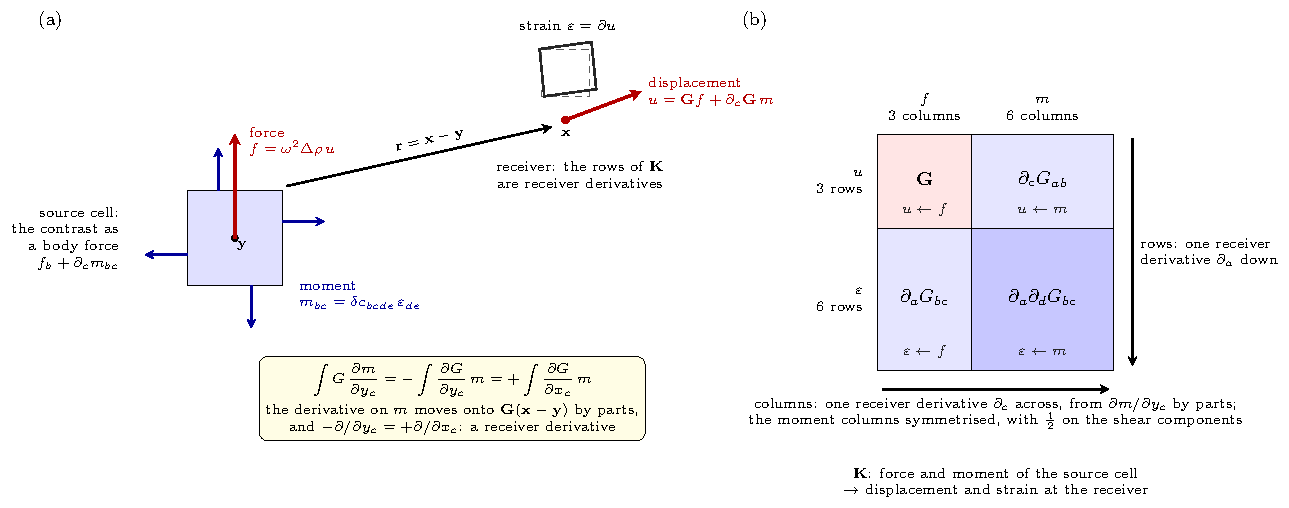
\includegraphics[width=\linewidth]{../figures/fig_kernel.pdf}
\caption{Where the kernel comes from. (a) A source cell at $\mathbf y$ acts on the background through
the body force of Eq.~\eqref{eq:bodyforce}: a force $f$ from its density contrast, and the divergence
of its contrast stress $m$, the moment, from its stiffness contrast (arrows on the faces). At the
receiver $\mathbf x$ the state is the displacement $u$ and the strain $\varepsilon$. The moment's
derivative moves onto $\bG(\mathbf x-\mathbf y)$ by parts, Eq.~\eqref{eq:byparts}, and becomes a
receiver derivative with a plus sign. (b) The block structure of the $9\times9$ kernel $\bK$ that
results: the force columns are $\bG$, the moment columns carry one receiver derivative across, the
strain rows one receiver derivative down, and the strain-from-moment block two.}
\label{fig:kernel}
\par\smallskip{\footnotesize\textit{Alt text:} Two panels. On the left, a shaded square cell with a
dot at its centre marked y; a thick red arrow labelled force rises from the centre, and four blue
arrows labelled moment point outward from the cell's faces. A long arrow labelled r equals x minus y
runs from the cell to a red dot marked x at the upper right, from which a red arrow labelled
displacement leaves and above which a small dashed square deformed into a parallelogram is labelled
strain. A boxed line below reads: the integral of G times the y-derivative of m equals minus the
integral of the y-derivative of G times m, equals plus the integral of the x-derivative of G times m.
On the right, a two-by-two grid of shaded blocks with rows labelled u, three rows, and strain, six
rows, and columns labelled f, three columns, and m, six columns; the blocks read G, the first
derivative of G, the first derivative of G, and the second derivative of G; an arrow down the right
side reads rows: one receiver derivative down, and an arrow along the bottom reads columns: one
receiver derivative across.\par}
\end{figure}

\paragraph{Averaging, and collocation} Three operations in this paper are averages over a cell,
and they are distinct. The \emph{source-cell average} integrates the kernel over the cell that
radiates: $\langle\bK\rangle(\mathbf r)=d^{-3}\int_{\text{cube}}\bK(\mathbf r-\mathbf y)\,\dd\mathbf y$
is the field at $\mathbf r$ of a uniform polarisation of the source cell. Every scheme in this paper
uses it, and \S\ref{sec:tiling} shows it to be exact. \emph{Collocation} fixes where the discrete
equation is imposed: at the receiving cell's centre, with the internal field of each cell uniform, so
that the unknown is the field at the centre. The \emph{receiver-cell average} imposes the equation in
the mean over the receiving cell instead; with a uniform internal field that is the Galerkin scheme
of degree zero, called the mean-only voxel below. The two are both \emph{uniform-field} voxels, a
term that refers to the internal field and not to the test, and they differ only in the test
function (a delta at the centre against the cell's indicator) and in the constant of their
$O((kd)^2)$ error (Table~\ref{tab:ratio}). The \emph{cell-mean contrast}, finally, is an average of
the material, not of the field: where the medium varies within a cell, the contrast is projected
onto the cell's basis, its mean for degree $r=0$, rather than sampled at the centre
(\S\S\ref{sec:hetero}, \ref{sec:sphere}). In the language of the coupled-dipole method, the point
dipole is collocation with the point kernel, the integrated Green tensor adds the source-cell
average, and the filtered coupled dipoles replace the point source by one of finite extent.

\paragraph{The laterally uniform layer} A layer of thickness $D$ is filled with $n$ planes of
voxels, $d=D/n$, and illuminated at normal incidence. The field is then laterally uniform, only the
zero-lateral-wavenumber (specular) component of the lattice coupling acts, and
Eq.~\eqref{eq:foldylax} becomes exactly a chain of $n$ planes coupled by the specular lattice sums
\begin{equation}\label{eq:specsum}
  \bS(m)=\sum_{\mathbf R}\bG(\mathbf R+m d\,\hat{\mathbf z}),
\end{equation}
where the sum runs over the lattice vectors $\mathbf R=d\,(0,p,q)$, $p,q$ integers, that join the centres of
the voxels in one plane (a square lattice of pitch $d$), and $m$ is the separation of the two planes in
units of $d$ (Fig.~\ref{fig:lattice}a,b). The question is whether, and how fast, this chain converges to the
continuous layer as $n\to\infty$ at fixed $D$.

\begin{figure}[t]
\centering
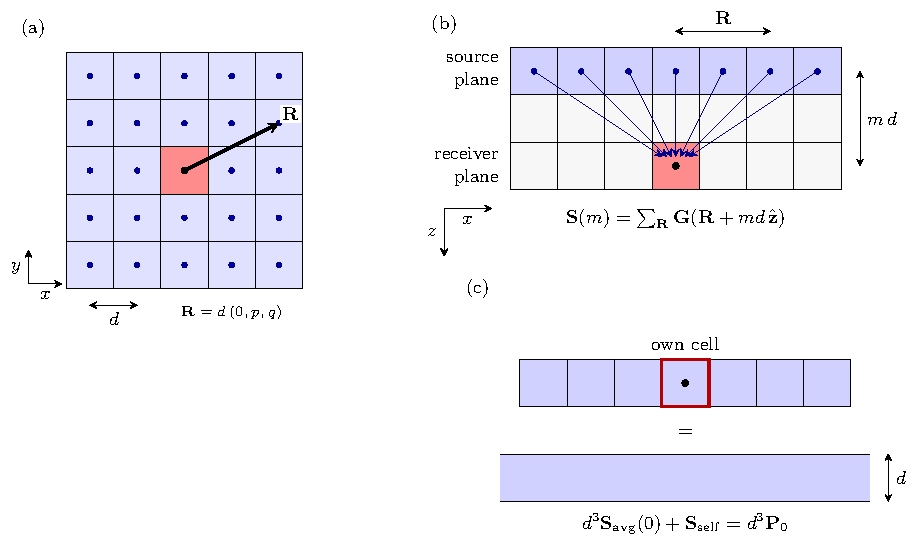
\includegraphics[width=\linewidth]{../figures/fig_lattice.pdf}
\caption{The lattice and its sums. (a) Plan view of one plane of voxels: their centres form a square
lattice of pitch $d$, and a lattice vector $\mathbf R=d\,(0,p,q)$ joins the centre of one voxel (shaded darker)
to another. (b) Cross-section ($z$ down), between planes: the voxel of a receiver plane (shaded darker) is coupled
to every voxel of a source plane $m$ planes above it, one for each lattice vector $\mathbf R$; the sum
over $\mathbf R$ is the specular lattice sum of Eq.~\eqref{eq:specsum}. (c) Within a plane: the sum
over every cell of the plane, the receiver's own cell (outlined) included, is the field of a uniform
plate of thickness $d$, the tiling identity of Eq.~\eqref{eq:tiling}.}
\label{fig:lattice}
\par\smallskip{\footnotesize\textit{Alt text:} Three schematic panels. On the left, a plan view of a
five-by-five grid of square voxels with a dot at each centre; the centre voxel is highlighted, an arrow
labelled R runs from its centre to another voxel centre, and the spacing between neighbouring centres is
marked d. At the top right, a cross-section through three rows of voxels: arrows from the centre of every
voxel in the top row converge on a highlighted voxel two rows below, with the plane separation m d
marked. Below it, a single row of voxels with one outlined as the receiver's own cell is shown equal
to a continuous shaded band of the same thickness d, a uniform plate.\par}
\end{figure}

\paragraph{Implementations} Every result is derived symbolically in Mathematica and compared with
an independent numerical implementation or an exact solution. ``The package'' below is the Python
implementation of the voxel scheme (\path{cubic_scattering}): its cube $T$-matrix, its lattice
kernels and its stratified propagator, which serve both as the object under test and, where
validated, as a second implementation.

\section{The continuous layer and its thin-layer expansion}\label{sec:continuum}

At normal incidence a plane force drives a one-dimensional problem per wave type, with modulus $M$
($M_P$ for P, $\mu$ for S), wavenumber $k$ and plane Green's function
$g(z)=\tfrac{\mathrm{i}}{2Mk}\mathrm{e}^{\mathrm{i}k|z|}$. The layer's reflection and transmission follow from continuity of
displacement and traction at its faces; they agree with the stratified propagator used as the
reference in this work to $2.5\times10^{-8}$, P and S (\path{ContinuumLimit_Reference.wl}).

For a layer of thickness $D$ with modulus $M_1$ and density $\rho_1$ in a background $M_0,\rho_0$,
write $Z_j=\sqrt{M_j\rho_j}$ for the impedances, $\zeta=Z_1/Z_0$ for their ratio and
$k_1=\omega\sqrt{\rho_1/M_1}$ for the layer's wavenumber. The reflection coefficient expands as
\begin{equation}\label{eq:thin}
\begin{aligned}
  R={}&\frac{\mathrm{i}k_1D}{2}\bigl(\zeta-\zeta^{-1}\bigr)
  +\frac{(k_1D)^2}{4}\bigl(\zeta^{-2}-\zeta^{2}\bigr)
  -\frac{\mathrm{i}(k_1D)^3}{24}\bigl(\zeta-\zeta^{-1}\bigr)\bigl(3\zeta^{-2}+2+3\zeta^{2}\bigr)\\
  &+\frac{(k_1D)^4}{48}\bigl(\zeta^{2}-\zeta^{-2}\bigr)\bigl(3\zeta^{2}-2+3\zeta^{-2}\bigr)+O(D^5),
\end{aligned}
\end{equation}
exact in the contrast (\path{ContinuumLimit_ThinLayer.wl}, which checks each coefficient symbolically
and the truncated series against the exact layer). The first term is
\begin{equation}\label{eq:thin1}
  \frac{\mathrm{i}\omega D}{2}\sqrt{\frac{M_0}{\rho_0}}
  \Bigl[\frac{\rho_1-\rho_0}{M_0}-\rho_0\Bigl(\frac1{M_1}-\frac1{M_0}\Bigr)\Bigr]:
\end{equation}
to first order a thin layer is an
interface across which the traction jumps by the excess inertia and the displacement by the excess
compliance. At oblique incidence the same statement holds with the first-order system
$\partial_z\mathbf b=\bA\mathbf b$ for the P--SV state $\mathbf b=(u_x,u_z,t_{xz},t_{zz})$: the layer
acts to $O(D)$ as the jump $\bI+(\bA_1-\bA_0)D$, which reproduces the layer's $O(D)$ reflection
coefficients $R_{PP},R_{PS}$ to $10^{-12}$; the series truncated at $O(D^k)$ converges at exactly
order $k$; and a soft thin layer with shear modulus $\mu_1=D/\eta$ at fixed compliance $\eta$ tends to
the linear-slip interface as $D\to0$. These expansions are the target a single plane of voxels must
reproduce order by order. A plane of voxels that carry Legendre moments of their internal field to
degree $p$ reproduces Eq.~\eqref{eq:thin} term by term through $O(D^{2p+2})$ and first differs at
$D^{2p+3}$ (\S\ref{sec:fourth}): the mean-only voxel reproduces the equivalent interface and the $D^2$
term, the first-moment voxel all four terms shown.

\section{The specular sums of the point Green's tensor}\label{sec:point}

\paragraph{Why transform the sum} The specular sum \eqref{eq:specsum} adds, at a receiver, the field
of every voxel of a plane $m$ planes away. In that form it is a poor object to study. The Green's
tensor decays slowly with distance, so the sum converges slowly, and it hides the one question that
matters here: which part of it is the continuum, and which part is the discretisation. The Poisson
summation formula \citep{SteinWeiss1971} answers both at once, and is the standard tool for lattice sums
of wave fields \citep{Linton2010}. For a function $f$ on the plane and the square lattice of pitch $d$
it states
\begin{equation}\label{eq:poissonformula}
  \sum_{\mathbf R}f(\mathbf R)=\frac1{d^2}\sum_{\mathbf g}\hat f(\mathbf g),\qquad
  \hat f(\mathbf g)=\int f(\mathbf x)\,\mathrm{e}^{-\mathrm{i}\mathbf g\cdot\mathbf x}\,\dd^2x,\qquad
  \mathbf g=\tfrac{2\pi}{d}(p,q),
\end{equation}
with $p,q$ integers: a sum of samples of $f$ on the lattice equals a sum of samples of its Fourier
transform on the reciprocal lattice, whose pitch is $2\pi/d$ (Fig.~\ref{fig:poisson}). Applied to the
specular sum,
\begin{equation}\label{eq:poisson}
  \bS(m)=\frac1{d^2}\sum_{\mathbf g}\hat\bG(\mathbf g;\,m d),
\end{equation}
with $\hat\bG(\mathbf g;z)$ the two-dimensional (lateral) transform of the Green's tensor between planes
a distance $z$ apart. Each term has a physical meaning. Transformed laterally, the field of a plane of
sources is a superposition of plane waves, one for each lateral wavenumber, and the lattice selects the
wavenumbers $\mathbf g$. The order $\mathbf g=0$ is the laterally uniform plane wave that a continuous
layer radiates: it is the continuum's term. Every other order has $|\mathbf g|\ge2\pi/d$, far beyond the
wavenumber of the field when the voxels are small compared with the wavelength, so it is evanescent and
decays away from the plane as $\mathrm{e}^{-|\mathbf g|md}=\mathrm{e}^{-2\pi m\sqrt{p^2+q^2}}$, independently
of $d$. The transform therefore splits the lattice sum exactly into the continuum and a discretisation
correction, and the correction converges after a few orders.

\begin{figure}[t]
\centering
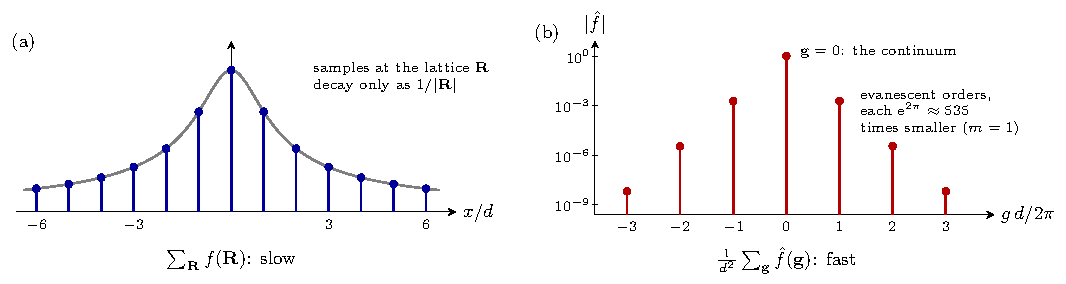
\includegraphics[width=\linewidth]{../figures/fig_poisson.pdf}
\caption{The Poisson summation formula \eqref{eq:poissonformula} applied to a plane of voxels, along one
lateral axis. (a) Real space: the field of each voxel of a source plane at a receiver one plane away,
sampled at the lattice points; the samples decay only as $1/|\mathbf R|$, so their sum converges
slowly. (b) The same sum after Poisson summation, on a logarithmic scale: samples of the lateral Fourier
transform at the reciprocal-lattice orders $\mathbf g=2\pi p/d$. The order $\mathbf g=0$ is the
continuum's plane wave; every other order is evanescent and, at $m=1$, smaller than its neighbour by
$\mathrm{e}^{2\pi}\approx535$. Magnitudes are schematic: the static decay $\mathrm{e}^{-|\mathbf g|md}$ is
shown.}
\label{fig:poisson}
\par\smallskip{\footnotesize\textit{Alt text:} Two panels. On the left, a smooth bell-shaped curve that
decays slowly on both sides is sampled by vertical stems at integer positions from minus six to six,
the stems remaining clearly visible far from the centre. On the right, on a logarithmic vertical axis
from one down to ten to the minus nine, a stem of height one at zero is labelled as the continuum, and
stems at plus and minus one, two and three fall by about three powers of ten per step and are labelled
as evanescent orders.\par}
\end{figure}

\paragraph{The local term that survives} In the strain-from-moment block the evanescent orders carry two
powers of $|\mathbf g|\propto1/d$, so their contribution per voxel volume does \emph{not} vanish as
$d\to0$: at $m=1$ it is eleven times the continuum term (\path{ContinuumLimit_SpecularSums.wl},
matched to the package's Ewald lattice sum to $5\times10^{-13}$). This surviving term is static.
Summed over all planes in slab order, the static lattice sum of the point kernel is exactly the
depolarisation of a uniform plate ($-1/M_P$ on $\varepsilon_{zz}\leftarrow M_{zz}$ and $-1/(2\mu)$
on the normal shears, per unit volume) plus a cubic-symmetric remainder
(\path{ContinuumLimit_StaticLocal.wl}, to $2\times10^{-10}$). The point kernel therefore reproduces
the continuum only if that remainder is cancelled by the voxel's own self term.

\section{The tiling identity}\label{sec:tiling}

Replace the point coupling by the \emph{source-cell average}
$\langle\bG\rangle(\mathbf r)=d^{-3}\int_{\text{cube}}\bG(\mathbf r-\mathbf y)\,\dd\mathbf y$, the
field at a voxel centre of a uniform polarisation of the source voxel. Each Poisson order in
Eq.~\eqref{eq:poisson} is then multiplied by the cube's form factor
\begin{equation}
  F(\mathbf g)=\sinc(g_x h)\,\sinc(g_y h),
\end{equation}
which vanishes at every $\mathbf g\neq0$ of the reciprocal lattice since $\sinc(p\pi)=0$ for integer
$p\neq0$. This is the Fourier form of the fact that cubes tile the plane,
$\sum_{\mathbf R}\chi(\mathbf x-\mathbf R)=1$ for the cube's indicator $\chi$: a partition of unity
(Fig.~\ref{fig:tiling}). Two exact statements follow.

\begin{figure}[t]
\centering
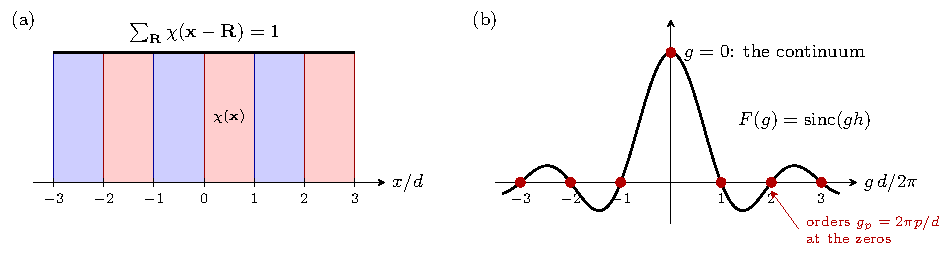
\includegraphics[width=\linewidth]{../figures/fig_tiling.pdf}
\caption{Why cubes make the coupling exact. (a) Cubes tile the plane: the indicator functions $\chi$ of
the translated cells sum to exactly one everywhere, a partition of unity. (b) The same fact in Fourier
space: the cube's lateral form factor $F(g)=\sinc(gh)$ (shown along one axis) vanishes at every
reciprocal-lattice order $g_p=2\pi p/d$ with $p\neq0$, so of all the orders in the lattice sum
\eqref{eq:poisson} only $g=0$, the continuum's plane wave, survives the source-cell average.}
\label{fig:tiling}
\par\smallskip{\footnotesize\textit{Alt text:} Two panels. On the left, adjacent box functions of unit
height and unit width, alternately shaded, lie side by side along an axis marked in voxel widths, and a
thick horizontal line at height one marks their sum. On the right, the sinc curve, equal to one at the
origin and oscillating with decaying amplitude, is plotted against wavenumber in units of $2\pi/d$; dots
mark the reciprocal-lattice orders, one at height one at the origin and all the others on the axis at
the zeros of the curve.\par}
\end{figure}

\paragraph{Between planes} For $m\neq0$ every evanescent order is removed and
\begin{equation}\label{eq:between}
  \bS_{\text{avg}}(m)=\frac1{d^2}\sum_{W=P,S}\hat\bG_W(0;\,m d)\,\sinc(k_W h),
\end{equation}
the continuum's plane-wave term times the vertical form factor. The package's cell-averaged kernel
agrees in all 81 entries to $2.8\times10^{-16}$ (\path{ContinuumLimit_AveragedSums.wl}).

\paragraph{Within a plane} The sum over \emph{all} cells of the plane, the voxel's own included,
is the field at the mid-plane of a uniform plate of thickness $d$ (Fig.~\ref{fig:lattice}c):
\begin{equation}\label{eq:tiling}
  d^3\,\bS_{\text{avg}}(0)+\bS_{\text{self}}=d^3\,\bP_0,
  \qquad
  \bS_{\text{self}}=\int_{\text{cube}}\bG(-\mathbf y)\,\dd\mathbf y,
\end{equation}
where $\bP_0=d^{-3}\int_{-h}^{h}\bG_{\text{plate}}(-z')\,\dd z'$ is elementary: in the one-dimensional
transform each entry is $c_0+A/(Mk_z^2-\rho\omega^2)$, so it averages to
$c_0/d+A\,(\mathrm{e}^{\mathrm{i}kh}-1)/(dMk^2)$. Its only nonzero entries are $u\leftarrow f$ on the diagonal and the
three normal strain-from-moment entries, whose local weights $-1/M_P$ and $-1/(2\mu)$ are the plate
depolarisation of \S\ref{sec:point}. Statically the identity holds for all 21 independent components
of the strain-from-moment tensor to $4\times10^{-9}$, with every cell integral evaluated analytically
(below).

\paragraph{Consequence: an exact kernel with no lattice sum} At normal incidence the same-plane
block of the cell-averaged Foldy--Lax kernel is
\begin{equation}\label{eq:exactkernel}
  \bS_{\text{avg}}(0)=\bP_0-\bS_{\text{self}}/d^3 ,
\end{equation}
with no Ewald splitting, near shell or asymptotic tail. The route it replaces (Ewald summation
with a near shell averaged by quadrature and an $O(d^2)$ Taylor tail beyond it) carries a static
strain-from-moment error of $9.4\times10^{-4}$ at its default settings, falling to $2.6\times10^{-5}$
only when both the shell radius and the quadrature order are raised; Eq.~\eqref{eq:exactkernel} is
now the package's kernel at normal incidence.

\paragraph{Cell integrals without quadrature} Write the static (Kelvin) tensor as
$G_{bc}=(c_A+c_B)\,\delta_{bc}/r-c_B\,\partial_b\partial_c r$ with
$c_B=(1/\mu-1/M_P)/8\pi$ and $c_A=1/(4\pi\mu)-c_B$. Every cell integral of its derivatives is a cell
integral of derivatives of $1/r$ and $r$. One application of the divergence theorem moves it onto
faces $x_p=c_p\pm h$, which never contain the origin, and there the two-dimensional antiderivative in
the face coordinates is continuous, so the face integral is a sum over the face's corners. The
distributional term at $r=0$ is carried by the divergence theorem itself. (A triple antiderivative
evaluated at the cube's corners is \emph{not} usable for repeated derivatives: its arctangent terms
jump across the coordinate planes through the origin, and differentiating twice there discards
exactly that term.) The self term so obtained reproduces the classical closed form of the cube's
depolarisation to machine precision.

\section{The single site: the cube \texorpdfstring{$T$}{T}-matrix from moment integrals}\label{sec:single}

Every error of a voxel scheme is made at the single site (\S\ref{sec:discussion}), so the single
site is derived here rather than imported. The classical route imports it. For an ellipsoid,
Eshelby's uniformity theorem makes the internal strain under a uniform load uniform, with a
depolarisation tensor in closed form \citep{Eshelby1957,Eshelby1959,Mura1987}; its dynamic
generalisation is known for spheres and ellipsoids \citep{Mikata1990,Michelitsch2003}. For a cube
or a general polyhedron the static field of a uniform eigenstrain is also in closed form
\citep{Chiu1977,LeeJohnson1978,Rodin1996,Nozaki2001}, but the strain it produces is not uniform,
so there is no exact uniform-strain inclusion to import. In scattering theory the same object
appears as the self-consistent or effective-field closure of the volume integral equation
\citep{MalKnopoff1967,Gubernatis1977,Kanaun2008}: a first-order (Born) scatterer
\citep{Wu1985} renormalised by the geometric series of its own near field, the step that turns a
contrast into an effective contrast. \citet{Nestor1996} introduced the single site in this form,
summing the series of the cell's self integral, with the singular near field evaluated over an
infinitesimal cell. The moments below evaluate the same self integral over the finite cube, as a
distribution. The elastic $T$-matrix of \citet{Waterman1976} represents a
scatterer in spherical multipoles, the natural basis for a sphere; a voxel in a lattice needs one
compatible with the lattice, and the moments over the cube provide it. The construction below makes the
approximation of a voxel explicit rather than implicit: it derives the cube's $T$-matrix from
the moments of the elastodynamic Green's tensor over the cube, and identifies the
uniform-strain closure as one truncation of an exact hierarchy.

\subsection{The closed hierarchy}\label{sec:hierarchy}

Let the voxel be $V=[-h,h]^3$ with contrast
$\delta c_{ijkl}=\Delta\lambda\,\delta_{ij}\delta_{kl}+\Delta\mu(\delta_{ik}\delta_{jl}+\delta_{il}\delta_{jk})$
and $\Delta\rho$. Expand the internal displacement about the centre to second degree and project
the Lippmann--Schwinger equation onto $1$, $x_p$ and $x_px_q$. The unknowns are $u_i(0)$,
$\partial_pu_i(0)$ and $\partial_p\partial_qu_i(0)$, and the result is the closed system
\begin{align}
\bigl(\delta_{ij}-\omega^2\Delta\rho\,\mathsf G_{ij}\bigr)u_j
  +\bigl(\mathsf N^{r}_{in,k}\,\delta c_{nksj}-\tfrac12\omega^2\Delta\rho\,\mathsf K^{rs}_{ij}\bigr)
  \partial_r\partial_su_j
  &= u^0_i, \label{eq:A11}\\
\bigl(\delta_{pr}\delta_{ij}+\omega^2\Delta\rho\,\mathsf N^{r}_{ij,p}
  -\mathsf M_{in,pk}\,\delta c_{nkrj}\bigr)\partial_ru_j
  &= \partial_pu^0_i, \label{eq:A22}\\
-\omega^2\Delta\rho\,\mathsf M_{ij,pq}\,u_j
  +\bigl(\delta_{qr}\delta_{ps}\delta_{ij}+\mathsf Q^{r}_{in,pqk}\,\delta c_{nksj}
  -\tfrac12\omega^2\Delta\rho\,\mathsf P^{rs}_{ij,pq}\bigr)\partial_r\partial_su_j
  &= \partial_p\partial_qu^0_i, \label{eq:A33}
\end{align}
all fields evaluated at the centre. Its coefficients are six moments of the background Green's
tensor $\bG$ over the voxel,
\begin{equation}\label{eq:moments}
\begin{aligned}
\mathsf G_{ij}&=\int_V G_{ij}\,\dd V, &
\mathsf K^{rs}_{ij}&=\int_V G_{ij}\,x_rx_s\,\dd V, &
\mathsf N^{r}_{in,k}&=\int_V \partial'_kG_{in}\,x_r\,\dd V,\\
\mathsf M_{in,pk}&=\int_V \partial'_p\partial'_kG_{in}\,\dd V, &
\mathsf P^{rs}_{ij,pq}&=\int_V \partial'_q\partial'_pG_{ij}\,x_rx_s\,\dd V, &
\mathsf Q^{r}_{in,pqk}&=\int_V \partial'_q\partial'_p\partial'_kG_{in}\,x_r\,\dd V,
\end{aligned}
\end{equation}
with derivatives taken with respect to the source point, $\partial'=-\partial$. That sign reaches
$\mathsf N$ and $\mathsf Q$ only, and no symmetry, parity or scaling check can detect it, so it is
fixed by convention. The moments are graded by $(D,W)$, the number of derivatives and the degree of
the weight: $\mathsf G\,(0,0)$, $\mathsf K\,(0,2)$, $\mathsf N\,(1,1)$, $\mathsf M\,(2,0)$,
$\mathsf P\,(2,2)$, $\mathsf Q\,(3,1)$.

\subsection{The moments as distributions}\label{sec:distributions}

Write the elastodynamic tensor as
\begin{equation}\label{eq:Gdecomp}
  G_{in}(\mathbf r)=\frac{1}{4\pi\mu}\Bigl[\delta_{in}\,g_{S}(r)
  +\frac{1}{k_S^2}\,\partial_i\partial_n\bigl(g_S(r)-g_P(r)\bigr)\Bigr],
  \qquad g_{c}(r)=\frac{\mathrm{e}^{\mathrm{i}k_cr}}{r}
\end{equation}
\citep{Kupradze1963,Aki2002}. Expanding $g_c$ in powers of $r$ reduces every moment in
Eq.~\eqref{eq:moments} to a finite sum of scalar moments
\begin{equation}\label{eq:Emoment}
  E\bigl[m;d_1\ldots d_D;w_1\ldots w_W\bigr]
  =\bigl\langle \partial_{d_1}\!\cdots\partial_{d_D}\,r^m,\ x_{w_1}\!\cdots x_{w_W}\,\mathbf 1_V\bigr\rangle .
\end{equation}
For $m=-1$ and $D\ge2$ the classical integrand is not absolutely integrable. $\partial^2(1/r)$
decays as $r^{-3}$, its angular average vanishes, and the value of the integral depends on the
shape of the region excluded around the origin. This is the source of the $\delta$-function term
of the inclusion problem, which a numerical quadrature misses. Without it the depolarisation is
wrong; for a sphere it vanishes altogether (\S\ref{sec:parity}). It is not added afterwards here. The derivatives are
distributional from the start, and each is moved onto the voxel's faces by pairing with the test
function $w\mathbf 1_V$, using $\partial_q\mathbf 1_V=-n_q\,\delta_{\partial V}$:
\begin{equation}\label{eq:peel}
  \bigl\langle \partial_qT,\,w\mathbf 1_V\bigr\rangle
  =\oint_{\partial V} n_q\,w\,T\,\dd A-\bigl\langle T,\,(\partial_qw)\,\mathbf 1_V\bigr\rangle .
\end{equation}
The surface term is evaluated on the faces, a distance $h$ from the origin, where every
derivative of $r^m$ is smooth. The recursion lowers $D$ and $W$ together and ends on convergent
integrals. The face integrals are done in closed form by the corner sums of \S\ref{sec:tiling}. The
sharp check is the sum rule
\begin{equation}\label{eq:sumrule}
  \textstyle\sum_pE[-1;p,p;\,]=\nabla^2(1/r)\ \text{paired with}\ \mathbf 1_V=-4\pi ,
\end{equation}
which the face route satisfies exactly and a spherical excision returns as $0$. The closed forms
contain logarithms of the units $(2\pm\sqrt3)^n$ of the Pell equation $x^2-3y^2=1$. Left
unreduced, these cancel catastrophically: for example, $\log(72010600134783751-41575339372323900\sqrt3)$
is a cancellation of $35$ digits. They are therefore reduced to $n\log(2-\sqrt3)$, which is
exact. Because every power of $r$ is paired this way, the dynamic moments keep the even-power terms
of the expansion ($k^2r$, $r^3$, \dots) as well as the odd ones. A route that integrates only the
polynomial (odd-power) terms of $\bG$ misses those terms, at a real $O((kh)^2)$ cost
(\S\ref{sec:closure}).

\subsection{Parity, and the nine-component block}\label{sec:parity}

The cube is centrosymmetric. A moment that couples a field quantity of degree $a$ to one of degree
$b$ therefore vanishes unless $a+b$ is even. $u$, $\partial u$ and $\partial\partial u$ have
degrees $0$, $1$ and $2$, so Eq.~\eqref{eq:A22} contains the first gradient alone: $\partial u$
is determined by its own block and couples to neither $u$ nor $\partial\partial u$. The leading
scattering by a stiffness contrast is the stress dipole $\int_V\delta c:\nabla u\,\dd V$, which needs
only $\partial u$. The leading far field of the stiffness contrast is therefore fixed by
Eq.~\eqref{eq:A22}, and \emph{no treatment of the second-gradient block \eqref{eq:A33} can change
it}. What Eq.~\eqref{eq:A33} contributes reaches the far field only through the $O((kh)^2)$
coupling in Eq.~\eqref{eq:A11}. That is the order, and the origin (the variation of the field
across the voxel), of the collocation error of \S\ref{sec:convergence}, which the first-moment
voxel of \S\ref{sec:fourth} removes.

With $\Delta\rho=0$, Eq.~\eqref{eq:A22} is the $9\times9$ operator
$\delta_{pr}\delta_{ij}-\mathsf M_{in,pk}\,\delta c_{nkrj}$, built from $\mathsf M$ alone. Under
$O_h$ the nine gradient components decompose as $A_{1g}\oplus E_g\oplus T_{1g}\oplus T_{2g}$, and
the operator is diagonal in that basis. Its eigenvalues are the inverse strain concentrations:
\begin{align}
A_{1g}\ \text{(dilatation)}:&\quad 1+\frac{\Delta\lambda+\tfrac23\Delta\mu}{\lambda+2\mu},
  \label{eq:A1g}\\
T_{2g}\ \text{(off-diagonal shear)}:&\quad 1+2\Delta\mu\,S_{\text{off}},\qquad
  S_{\text{off}}=\frac{\pi(\lambda+2\mu)-\sqrt3\,(\lambda+\mu)}{3\pi\mu(\lambda+2\mu)},
  \label{eq:T2g}\\
E_{g}\ \text{(diagonal shear)}:&\quad 1+2\Delta\mu\,S_{\text{diag}},\qquad
  S_{\text{diag}}=\frac{3\sqrt3\,(\lambda+\mu)+2\pi\mu}{6\pi\mu(\lambda+2\mu)}.
  \label{eq:Eg}
\end{align}
The density channel is the displacement block of Eq.~\eqref{eq:A11} with the second gradients
dropped, an amplification $(1-\omega^2\Delta\rho\,\mathsf G)^{-1}$ with $\mathsf G$ the cube
integral of $\bG$.

\paragraph{The cube against the sphere} For a sphere, Eshelby's tensor gives a dilatational
channel $1+\Delta K/(\lambda+2\mu)$, with $\Delta K=\Delta\lambda+\tfrac23\Delta\mu$, and a single
deviatoric channel $1+2\Delta\mu\,S_{\text{sph}}$, with $2\mu S_{\text{sph}}=2(4-5\nu)/[15(1-\nu)]$.
The cube's dilatational channel, Eq.~\eqref{eq:A1g}, is the sphere's exactly: its eigenvalue
involves $\mathsf M$ only through the contraction $\int_V\partial_i\partial_nG_{in}\,\dd V$, and the
static Navier equation makes $\partial_i\partial_nG_{in}=-\delta(\mathbf r)/(\lambda+2\mu)$, whose
integral does not depend on the shape. The
cube's shear channels differ from each other. Their isotropic average, however, is the sphere's,
also exactly:
\begin{equation}\label{eq:shearsplit}
  \tfrac15\bigl(3S_{\text{off}}+2S_{\text{diag}}\bigr)=S_{\text{sph}},\qquad
  S_{\text{diag}}-S_{\text{off}}=\frac{(\lambda+\mu)(5\sqrt3-2\pi)}{6\pi\mu(\lambda+2\mu)}>0 .
\end{equation}
The $\sqrt3$ terms cancel in the average. What a cube adds to a sphere at this order is therefore
a pure cubic anisotropy. It splits the deviatoric channel about the sphere's value, weighted $3:2$
by the dimensions of $T_{2g}$ and $E_g$, and the diagonal shear is the more depolarised. At the background of
\S\ref{sec:convergence} ($\nu=7/32$), $2\mu S_{\text{off}}=0.4314$, $2\mu S_{\text{diag}}=0.5929$
and the sphere's value is $0.4960$.

\paragraph{Where Eshelby enters} Equations \eqref{eq:A1g}--\eqref{eq:Eg} follow from the moment
integrals and the group theory alone. No ellipsoidal result is used, and no $\delta$ term is added
by hand. What corresponds to Eshelby is the \emph{truncation}. Keeping $\partial u$ and discarding
$\partial\partial u$ is exactly the uniform-internal-strain ansatz, and by the uniformity theorem
that ansatz is exact if and only if the inclusion is an ellipsoid. For a sphere the construction
is therefore exact in the static limit, and for a cube it is an approximation. The hierarchy
\eqref{eq:A11}--\eqref{eq:A33} states that approximation as the omitted blocks, rather than as an
unquantified shape correction. A polynomial expansion about the centre cannot represent the edge
and corner concentrations of an isolated cube's internal field at any finite degree. A voxel in a
uniform layer has no such concentrations: its neighbours have the same properties, so its internal
field is the continuum's, which is smooth. That is why a low-degree internal field suffices in a
lattice (\S\S\ref{sec:convergence}--\ref{sec:fourth}) although it is only an approximation for an
isolated cube.

\paragraph{Against the exact sphere} These statements are tested against the exact elastic Mie
solution for a sphere, with no Eshelby formula in between. The concentration of Mie order $n$ is
$E_n=a_n/a_n^{\text{Born}}$ (orders $0$, $1$, $2$ are the dilatational, density and shear
channels), extrapolated to $ka\to0$. The formulation is applied to a ball of radius $a$, with its moment
$\mathsf M$ evaluated by the surface route of Eq.~\eqref{eq:peel} on $|\mathbf r|=a$. Its
dilatational and shear channels equal Mie's to $2\times10^{-10}$, and the density channel is
$1$. The cube's closed forms meet the same numbers. Its dilatational channel is Mie's
$E_0$ to $2\times10^{-10}$, and its isotropic shear average, Eq.~\eqref{eq:shearsplit}, is the
depolarisation read from Mie's $E_2$ to $10^{-8}$. The same moment taken as a principal value, over
the ball with a small sphere excluded around the origin, has zero depolarisation in every
channel. The whole static response of the sphere is the $\delta$ term.

At finite frequency the closure uses the dynamic ball moments, which are in closed form. It
departs from Mie at second order in $ka$ and first order in the contrast, and the departure is
closed-form too: the ball's moments are elementary, and Mie's low-frequency series with the
contrast kept exact gives $E_n$ to relative order $(ka)^3$. To first order in the contrast,
\begin{equation}\label{eq:spheredynamic}
\frac{E_n^{\text{closure}}}{E_n^{\text{Mie}}}-1=
\begin{cases}
  -\dfrac{(k_Pa)^2}{10}\,\dfrac{\Delta\lambda}{\lambda+2\mu}, & n=0,\\[8pt]
  \dfrac{2(k_Sa)^2+(k_Pa)^2}{30}\,\dfrac{\Delta\rho}{\rho}, & n=1,\\[8pt]
  -\dfrac{3(k_Sa)^2+2(k_Pa)^2\beta^2/\alpha^2}{75}\,\dfrac{\Delta\mu}{\mu}, & n=2,
\end{cases}
\end{equation}
with no $O(ka)$ term and no $O((ka)^3)$ term. The imaginary $(ka)^3$ terms, the radiation damping,
agree exactly in all three channels. So the closure's only error at this order is the real
$(ka)^2$ term, the uniform-field ansatz's own. That is the order the hierarchy assigns to the
omitted second gradients (\S\ref{sec:parity}), and it has the same origin, the variation of the
field across the scatterer, as the collocation error of \S\ref{sec:convergence}. Eq.~\eqref{eq:spheredynamic} is derived symbolically
(\path{SphereClosureDynamic.wl}). It agrees with the coefficient extracted from the numerical Mie
solve and an independent implementation of the closure to $5\times10^{-4}$, which is the size of the
next order in the contrast.

\subsection{The collocation closure}\label{sec:closure}

The collocation closure takes the internal field of a voxel as uniform, the truncation of
\S\ref{sec:parity} for the density and stiffness channels together. The voxel's own field at its
centre is then $\bS_{\text{self}}\bD\,e$ for internal state $e$, where $\bS_{\text{self}}$ is the
nine-component form of the moments $\mathsf G$ and $\mathsf M$. By parity it is block-diagonal. So
$e=\psi+\bS_{\text{self}}\bD e$ and
\begin{equation}\label{eq:closure}
  \bT=d^3\,\bD\bigl(\bI-\bS_{\text{self}}\bD\bigr)^{-1}.
\end{equation}
With the kernel \eqref{eq:exactkernel} the self term cancels. Substituting
$\psi=(\bI-\bS_{\text{self}}\bD)e$ into Eq.~\eqref{eq:foldylax},
\begin{equation}\label{eq:collocation}
  e_i=\psi^0_i+d^3\sum_j \bK_{\text{all}}(i,j)\,\bD\,e_j,
  \qquad
  \bK_{\text{all}}(i,i)=\bP_0,\quad \bK_{\text{all}}(i,j)=\bS_{\text{avg}}(i-j),
\end{equation}
an identity checked on the matrices to $4\times10^{-16}$. Every block of $\bK_{\text{all}}$ is an
\emph{exact} cell integral of the one-dimensional continuum kernel (Eqs.~\eqref{eq:between},
\eqref{eq:tiling}), so Eq.~\eqref{eq:collocation} is precisely the collocation of the continuum
Lippmann--Schwinger equation with a strain piecewise constant over voxels. It does not contain
$\bS_{\text{self}}$ at all.

The package's cube $T$-matrix is this closure statically: both blocks agree with
Eq.~\eqref{eq:closure} to $2\times10^{-5}$ at $k_Sh=0.01$, the difference falling
as $(kh)^2$ (\path{ContinuumLimit_CubeT.wl}). It departs dynamically by about $0.25(kh)^2$ through its
far-field form-factor corrections. Its self integrals are exact in the static and radiation parts
but omit the real even-power terms of the Green's tensor's expansion ($k^2r$, $r^3$, \dots), an
error of $0.4$--$0.6\,(kh)^2$ against the analytic self term, whose series agrees with the
closed-form elastodynamic tensor to $10^{-14}$. By Eq.~\eqref{eq:collocation} that error cannot enter
the closure scheme.

\section{Convergence, and the closed-form error}\label{sec:convergence}

\paragraph{Second order} For a layer $D=2$\,m with the contrast
$\Delta\lambda=2$\,GPa, $\Delta\mu=1$\,GPa, $\Delta\rho=100$\,kg\,m$^{-3}$ in a background
$\alpha=5000$, $\beta=3000$\,m\,s$^{-1}$, $\rho=2500$\,kg\,m$^{-3}$, illuminated by a P plane force,
the reflected displacement of the chain converges to the continuous layer's at order $2.000$ for
$n=4\to16$ at $\omega=60$, $300$ and $600$\,rad\,s$^{-1}$, with the collocation
\eqref{eq:collocation} and with the package $T$-matrix alike (\path{ContinuumLimit_Chain.wl}). The
error depends on $k_Sh$ alone. Throughout, an order quoted for a pair of grids is the apparent order
$\ln(e_1/e_2)/\ln(n_2/n_1)$ between them, with $e$ the relative error against the exact solution
and $n$ the refinement; the orders in the legend of Fig.~\ref{fig:convergence} are least-squares
slopes of $\ln e$ against $\ln n$ over the grids marked as fitted, with their standard errors. The
two agree where a sequence is asymptotic and differ where it is not, which the apparent orders show.

\paragraph{The leading error in closed form} In Eq.~\eqref{eq:collocation} the kernel is
integrated exactly; the only approximation is the internal field's variation across a voxel. At
first order in the contrast the discrete scattered field is therefore a midpoint rule applied to
the continuum's Born integral, with the kernel's cell integral exact. For reflection the integrand
carries the two-way phase $\mathrm{e}^{2\mathrm{i}kz}$; for transmission it is flat. With $k$ the background
wavenumber of the wave concerned ($k_P$ for an incident P wave, $k_S$ for an incident S wave), $R$ the reflection coefficient and $T^{\text{sc}}$ the
scattered part of the transmitted field, for \emph{every} $n$
\begin{equation}\label{eq:errorR}
  \frac{R_{\text{disc}}}{R}=\frac{\sinc(kh)}{\sinc(2kh)}=1+\frac{(kd)^2}{8}+O(d^4),
  \qquad
  \frac{T^{\text{sc}}_{\text{disc}}}{T^{\text{sc}}}=\sinc(kh)=1-\frac{(kd)^2}{24}+O(d^4),
\end{equation}
confirmed for $n=1$ to $16$ to $10^{-4}$ of the error itself
(\path{ContinuumLimit_ErrorConstant.wl}); for an incident S wave, with $k=k_S$, the same forms and those of
Eq.~\eqref{eq:ratio} hold to $4\times10^{-4}$ (\path{ContinuumLimit_IncidentS.wl}, \S\ref{sec:fourth}). At the full contrast the reflection constant is unchanged
($0.124$ against $1/8$); the transmission constant grows to $-0.092$.

\paragraph{Why a uniform-field single site stops at second order} The two constants have opposite
signs, so no scalar correction of $\bT$, no single $O((kh)^2)$ factor, can cancel both. The
package $T$-matrix illustrates it: its form-factor corrections reduce the reflection error by a
factor $4.45$ and \emph{increase} the transmission error by $1.7$, at every $n$. The missing term in
Eq.~\eqref{eq:errorR} is the first moment of the internal field over each voxel, which radiates
through the derivative of the kernel. A fourth-order scheme must carry it: a single site with a
gradient channel, and a kernel whose cell integrals include the kernel's derivative.

\section{Fourth order and beyond: Legendre moments of the voxel field}\label{sec:fourth}

Let each voxel carry the mean \emph{and} the first moment of its internal field. On voxel $j$, with
local coordinate $s\in[-h,h]$ and Legendre functions $\phi_b(s)=P_b(s/h)$ ($\phi_0=1$, $\phi_1=s/h$,
$\phi_2=(3s^2/h^2-1)/2$, \dots), the field is
$w=\sum_{b}c_{b,j}\,\phi_b$, $w=(u,\varepsilon)$ the displacement and strain of the P channel, and
the polarisation is $q=(\omega^2\Delta\rho\,u,\ \Delta M\,\varepsilon)$ with $\Delta M=\Delta\lambda
+2\Delta\mu$. Testing the continuum equation
\begin{equation}
  w(z)=w^0(z)+\int\bK(z-z')\,q(z')\,\dd z',\qquad
  \bK=\begin{pmatrix} g & g' \\ g' & g''\end{pmatrix},\quad g''=-k^2g-\delta(z)/M_P,
\end{equation}
with the same functions on every voxel gives
\begin{equation}\label{eq:galerkin}
  \Bigl(\int_{i}\phi_a^2\,\dd z\Bigr)c_{a,i}
  =\int_i\phi_a w^0\,\dd z+\sum_{j,b}\Bigl[\int_i\!\!\int_j\phi_a(z)\,\bK(z-z')\,\phi_b(z')\,\dd z\,\dd z'\Bigr]
  \bD_1 c_{b,j},
\end{equation}
$\bD_1=\operatorname{diag}(\omega^2\Delta\rho,\Delta M)$. Between voxels the double integral is
separable, a product of Legendre moments of $\mathrm{e}^{\pm \mathrm{i}kz}$; within a voxel it is split at $z'=z$ and
the local term contributes $-\int_i\phi_a\phi_b\,\dd z/M_P$. Every entry is closed-form. Keeping only
$\phi_0$ recovers a second-order scheme; keeping $\phi_0$ and $\phi_1$ converges at fourth order in
both reflection and transmission (\path{ContinuumLimit_FourthOrder.wl}; Table~\ref{tab:fourth1d}).
\begin{table}[htbp]
\centering
\caption{Relative error of the scattered displacement of the layer, reflection / transmission, at $\omega=300$\,rad\,s$^{-1}$, against the number of voxel planes $n$: collocation, the mean-only voxel and the first-moment voxel of Eq.~\eqref{eq:galerkin}. The order is $4.00$ at $\omega=60$ and $600$\,rad\,s$^{-1}$ too.}\label{tab:fourth1d}
\begin{tabular}{@{}rccc@{}}
\toprule
$n$ & collocation & mean only & mean and first moment \\
\midrule
$1$  & $1.8\times10^{-3}$ / $1.3\times10^{-3}$ & $1.2\times10^{-3}$ / $1.8\times10^{-3}$ &
       $2.8\times10^{-7}$ / $2.8\times10^{-7}$ \\
$4$  & $1.1\times10^{-4}$ / $8.3\times10^{-5}$ & $7.5\times10^{-5}$ / $1.1\times10^{-4}$ &
       $1.1\times10^{-9}$ / $1.1\times10^{-9}$ \\
$16$ & $7.0\times10^{-6}$ / $5.2\times10^{-6}$ & $4.7\times10^{-6}$ / $6.9\times10^{-6}$ &
       $4.2\times10^{-12}$ / $4.2\times10^{-12}$ \\
order & $2$ / $2$ & $2$ / $2$ & $4$ / $4$ \\
\bottomrule
\end{tabular}
\end{table}
A single plane of first-moment
voxels represents the $2$\,m layer $6500$ times more accurately than a single plane of uniform ones.
The collocation column is the scheme of \S\ref{sec:single} and reproduces the chain of the full
$9\times9$ system to all printed digits.

\paragraph{Higher moments} Carrying the Legendre moments to degree $p$ changes nothing in the
construction: the moments and the same-cell double integrals of $P_b(s/h)$ against exponentials are
again closed-form, and for $p\le1$ the general-degree solver reproduces the chain above exactly. The
second-moment voxel ($p=2$) converges at sixth order and the third-moment voxel ($p=3$) at eighth, in
reflection and transmission (Table~\ref{tab:higher}; \path{ContinuumLimit_SecondMoment.wl}); the
second-moment voxel's order is $6.00$ at $\omega=60$, $300$ and $600$\,rad\,s$^{-1}$. The errors fall to
$10^{-22}$, so they are computed in 40-digit arithmetic.
\begin{table}[htbp]
\centering
\caption{Relative error of the scattered displacement of the layer, reflection / transmission, at
$\omega=300$\,rad\,s$^{-1}$, for voxels carrying Legendre moments to degree $p$. The order is the mean
over the halvings $n=2\to4\to8$.}\label{tab:higher}
\small\setlength{\tabcolsep}{4pt}
\begin{tabular}{@{}rccc@{}}
\toprule
$n$ & first moment ($p=1$) & second moment ($p=2$) & third moment ($p=3$) \\
\midrule
$1$ & $2.8\times10^{-7}$ / $2.8\times10^{-7}$ & $2.8\times10^{-11}$ / $4.2\times10^{-11}$ &
      $1.5\times10^{-15}$ / $1.5\times10^{-15}$ \\
$2$ & $1.7\times10^{-8}$ / $1.7\times10^{-8}$ & $4.4\times10^{-13}$ / $6.5\times10^{-13}$ &
      $6.0\times10^{-18}$ / $6.0\times10^{-18}$ \\
$4$ & $1.1\times10^{-9}$ / $1.1\times10^{-9}$ & $6.9\times10^{-15}$ / $1.0\times10^{-14}$ &
      $2.4\times10^{-20}$ / $2.4\times10^{-20}$ \\
$8$ & $6.7\times10^{-11}$ / $6.7\times10^{-11}$ & $1.1\times10^{-16}$ / $1.6\times10^{-16}$ &
      $9.2\times10^{-23}$ / $9.2\times10^{-23}$ \\
order & $4$ / $4$ & $6$ / $6$ & $8$ / $8$ \\
\bottomrule
\end{tabular}
\end{table}

\paragraph{The leading error in closed form} Without scattering, the Galerkin solution is the
$L^2$ projection $\Pi$ of the incident field onto each voxel's basis, and the kernel is integrated
over each voxel exactly; at first order in the contrast the error is therefore the kernel's cell
integral applied to $\Pi w^0-w^0$. The field varies as $\mathrm{e}^{\mathrm{i}ks}$ across a voxel and the kernel toward
an outside observer as $\mathrm{e}^{\mathrm{i}qs}$, $q=+k$ for reflection and $q=-k$ for transmission, so for every
scheme and every $n$
\begin{equation}\label{eq:ratio}
  \frac{\text{discrete}}{\text{exact}}
  =\frac{\int_{-h}^{h}\mathrm{e}^{\mathrm{i}qs}\,\Pi[\mathrm{e}^{\mathrm{i}ks}]\,\dd s}{\int_{-h}^{h}\mathrm{e}^{\mathrm{i}(q+k)s}\,\dd s},
\end{equation}
with $\Pi$ the centre value for collocation, the cell mean for the mean-only voxel and the projection
onto $\{P_0,\dots,P_p\}$ for the voxel of degree $p$ (\path{ContinuumLimit_FourthOrderError.wl},
\path{ContinuumLimit_SecondMoment.wl}). The results are in Table~\ref{tab:ratio}.
\begin{table}[htbp]
\centering
\caption{The leading error of the discrete layer in closed form, Eq.~\eqref{eq:ratio}: discrete over exact scattered field at first order in the contrast, for every number of voxel planes $n$.}\label{tab:ratio}
\begin{tabular}{@{}lcc@{}}
\toprule
 & reflection & transmission \\
\midrule
collocation      & $1+(kd)^2/8+O(d^4)$  & $1-(kd)^2/24+O(d^4)$ \\
mean only        & $1+(kd)^2/12+O(d^4)$ & $1-(kd)^2/12+O(d^4)$ \\
first moment     & $1-(kd)^4/720+O(d^6)$ & $1-(kd)^4/720+O(d^6)$ \\
second moment    & $1+(kd)^6/100800+O(d^8)$ & $1-(kd)^6/100800+O(d^8)$ \\
third moment     & $1-(kd)^8/25401600+O(d^{10})$ & $1-(kd)^8/25401600+O(d^{10})$ \\
degree $p$       & $1+(-1)^pc_p(kd)^{2p+2}$ & $1-c_p(kd)^{2p+2}$ \\
\bottomrule
\end{tabular}
\end{table}
The chain of Eq.~\eqref{eq:galerkin} reproduces the forms for collocation and degrees $0$ and $1$
at $n=1$ to $8$ to $10^{-4}$ of the error, the remainder being the second order in the contrast, and
those for degrees $2$ and $3$ to $4\times10^{-7}$ at a contrast reduced by $10^{-6}$. The constant for
degree $p$ follows from the Legendre expansion
$\mathrm{e}^{\mathrm{i}ks}=\sum_j\mathrm{i}^j(2j+1)\,j_j(kh)\,P_j(s/h)$. The projection drops the terms
$j>p$, led by $j=p+1$, whose coefficient is $O\bigl((kh)^{p+1}\bigr)$; its moment against
$\mathrm{e}^{\mathrm{i}qs}$ is $2h\,\mathrm{i}^{p+1}j_{p+1}(qh)=O\bigl((qh)^{p+1}\bigr)$. With
$j_n(x)\approx x^n/(2n+1)!!$ and $h=d/2$,
\begin{equation}\label{eq:cp}
  c_p=\frac{2p+3}{4^{p+1}\bigl[(2p+3)!!\bigr]^2}=\frac{\bigl[(p+1)!\bigr]^2}{(2p+2)!\,(2p+3)!},
  \qquad c_0=\tfrac1{12},\ c_1=\tfrac1{720},\ c_2=\tfrac1{100800},
\end{equation}
and the leading error carries $(q/k)^{p+1}$: the same sign in reflection and transmission for odd
$p$, opposite signs for even $p$. The first-moment voxel's leading error therefore does not depend on
the direction in which the field is observed. Eq.~\eqref{eq:cp} is checked symbolically for $p=0$ to
$5$ (every lower power of $kd$ vanishes) in Mathematica and, independently, in sympy.

\paragraph{One plane of voxels and the thin-layer series} Refining at fixed thickness is one limit;
thinning a single plane is the other. For one plane of voxels ($n=1$, $d=D$) the series in $D$ of the
reflection coefficient, computed exactly at the full contrast, coincides with that of the exact layer,
Eq.~\eqref{eq:thin}, term by term through $D^{2p+2}$ and first differs at $D^{2p+3}$, for $p=0$ to $3$
and for a layer both stiffer and softer than its surroundings (\path{ContinuumLimit_SecondMoment.wl}).
Each further Legendre moment adds two terms of the thin-layer series.

\paragraph{In three dimensions} The three-dimensional first-moment voxel carries the nine-component
state with Legendre weights $\{1,\,x/h,\,y/h,\,z/h\}$, 36 unknowns in all, tested with the same
functions and coupled by cell-to-cell double integrals of the Green's tensor. For a laterally uniform
layer at normal incidence it reduces \emph{exactly} to Eq.~\eqref{eq:galerkin}
(\path{ContinuumLimit_Reduction3D.wl}). The lateral first moments are never excited: the lattice and
the incident field are symmetric under reflection about every voxel's centre planes, and $x/h$, $y/h$
are odd there. The mean and the $z$-moment carry weights that are constant laterally, so their lateral
form factor $\sinc(g_xh)\sinc(g_yh)$ vanishes on the reciprocal lattice and the plane sum of the
double integrals is the plate-to-plate integral in $z$ alone. Two facts mark where genuinely
three-dimensional structure begins. The lateral first moment's form factor,
$F_1(g)=\mathrm{i}\,(gh\cos gh-\sin gh)/(gh)^2$, does not vanish on the reciprocal lattice
($F_1=\mathrm{i}(-1)^p/p\pi$), so the gradient channels couple through the evanescent orders. And at oblique
incidence the mean's own zeros shift, $\sinc\bigl((2\pi p/d+k_x)h\bigr)=(-1)^p k_xh/p\pi+O(k_x^2h^2)$,
so the tiling identity holds only to $O(k_\parallel h)$.

\paragraph{Oblique incidence} The scheme is built spectrally. By Poisson summation the Bloch coupling
between planes $i$ and $j$ at lateral wavenumber $\mathbf k_\parallel$ is
\begin{equation}\label{eq:bloch}
  C_{ab}(i,j)=\frac1{d^2}\sum_{\mathbf g}L_a(\boldsymbol\kappa)\,L_b(-\boldsymbol\kappa)\,
  \int\!\!\int\phi_a(z)\,\hat\bG(\boldsymbol\kappa;z-z')\,\phi_b(z')\,\dd z\,\dd z',
  \qquad \boldsymbol\kappa=\mathbf k_\parallel+\mathbf g,
\end{equation}
with $L_a$ the lateral Legendre factors. The whole-space tensor decays as $1/k_z^2$ and the nine-component
state adds at most two powers of $k_z$, so each entry of $\hat\bG(\boldsymbol\kappa;z)$ is a $\delta(z)$
of constant weight plus, per mode, $[\mathrm{i}\alpha/2\gamma+\mathrm{i}\beta\,\mathrm{sgn}(z)/2]\,\mathrm{e}^{\mathrm{i}\gamma|z|}$,
$\gamma^2=k_W^2-\kappa^2$: every $z$ integral is closed-form. Double averaging makes the lattice sum
converge without Ewald splitting, to three digits at $|p|,|q|\le8$. Against the exact layer, for a P
wave incident at $20^\circ$ and $40^\circ$ (\path{ContinuumLimit_Oblique.wl}; Table~\ref{tab:oblique}).
\begin{table}[htbp]
\centering
\caption{Relative error of the reflected P ($R_{PP}$) and converted S ($R_{PS}$) waves for a P wave incident at $20^\circ$, with the mean-only and first-moment voxels of Eq.~\eqref{eq:bloch}. At $40^\circ$ the orders are again $2$ and $4$.}\label{tab:oblique}
\small\setlength{\tabcolsep}{4pt}
\begin{tabular}{@{}rcccc@{}}
\toprule
 & \multicolumn{2}{c}{mean only} & \multicolumn{2}{c}{mean and first moments}\\
$n$ & $R_{PP}$ & $R_{PS}$ & $R_{PP}$ & $R_{PS}$ \\
\midrule
$1$ & $9.3\times10^{-4}$ & $1.7\times10^{-3}$ & $7.2\times10^{-8}$ & $4.1\times10^{-7}$ \\
$2$ & $2.3\times10^{-4}$ & $4.2\times10^{-4}$ & $4.5\times10^{-9}$ & $2.5\times10^{-8}$ \\
$8$ & $1.5\times10^{-5}$ & $2.7\times10^{-5}$ & $1.7\times10^{-11}$ & $9.9\times10^{-11}$ \\
order & $2$ & $2$ & $4$ & $4$ \\
\bottomrule
\end{tabular}
\end{table}
The mean-only voxel is
second order and the first-moment voxel fourth order in both the reflected P and the converted S wave:
the breakdown of the tiling identity at $O(k_\parallel h)$ and the evanescent coupling of the gradient
channels do not cost an order. At $\mathbf k_\parallel=0$ the construction reproduces
Eq.~\eqref{eq:galerkin} to all printed digits.

\paragraph{Incident S} Nothing in the construction is specific to P. For a normally incident S wave
the layer is the one-dimensional problem of Eq.~\eqref{eq:galerkin} with $M_P\to\mu$, $k_P\to k_S$ and
$\Delta M\to\Delta\mu$; the collocation and mean-only schemes converge at order $2.00$ and the
first-moment voxel at $4.00$, in reflection and transmission, and the full $9\times9$ construction
with an incident SH wave reproduces that one-dimensional result to all printed digits. At oblique
incidence, against the exact layer (\path{ContinuumLimit_IncidentS.wl}), the orders are those of
Table~\ref{tab:incS}.
\begin{table}[htbp]
\centering
\caption{Observed order of convergence ($n=2\to8$, $\omega=300$\,rad\,s$^{-1}$) for incident SV and SH waves, with the mean-only and first-moment voxels. The SV angles lie below the critical angle $\arcsin(\beta/\alpha)=36.9^\circ$.}\label{tab:incS}
\small
\begin{tabular}{@{}lcc@{}}
\toprule
 & mean only & mean and first moments \\
\midrule
SV at $20^\circ$: $R_{SS}$ / $R_{SP}$ & $2.00$ / $2.00$ & $4.00$ / $3.99$ \\
SV at $30^\circ$: $R_{SS}$ / $R_{SP}$ & $1.98$ / $2.00$ & $3.97$ / $4.00$ \\
SH at $20^\circ$ and $40^\circ$: $R_{SH}$ & $2.00$ & $4.00$ \\
\bottomrule
\end{tabular}
\end{table}
The orders, and with $k=k_S$ the closed-form constants of
Eqs.~\eqref{eq:errorR} and \eqref{eq:ratio}, are those of the incident P wave.

\paragraph{Degree two at oblique incidence} In three dimensions the voxel of degree $2$ carries, on each
of the nine components of its state, the ten Legendre products of total degree at most two in
$(z,x,y)$. In the construction of Eq.~\eqref{eq:bloch} it converges at sixth order against the exact
layer for incident P, SV and SH waves (Table~\ref{tab:deg2}; \path{scripts/measure_oblique_degree.py}).
The test is run at $\omega=3000$\,rad\,s$^{-1}$ ($k_PD=1.2$, $k_SD=2$), ten times the frequency of the
other tables, because at $300$\,rad\,s$^{-1}$ a sixth-order error on these grids lies below the round-off
of double precision. The exact reflection coefficient is that of Kennett's recursion, an independent
algorithm, and the same computation with the bases of degree $0$ and $1$ returns orders $2$ and $4$ in
all five cases. At normal incidence the error on four planes, $6.95\times10^{-9}$, is the
$c_2(kd)^6=7.2\times10^{-9}$ of Eq.~\eqref{eq:cp} to $4\%$. Doubling the number of lattice orders retained
in Eq.~\eqref{eq:bloch} changes the errors by less than $1\%$. Unlike the degrees $0$ and $1$, this degree
is implemented once at oblique incidence; its check is the exact solution.
\begin{table}[htbp]
\centering
\caption{The voxel of degree $2$ (ten Legendre products per state component) at
$\omega=3000$\,rad\,s$^{-1}$: relative error of the same-type reflection coefficient against the exact
layer on $n$ planes, and the order over the last halving, with the orders of the degrees $0$ and $1$ from
the same computation.}\label{tab:deg2}
\small
\begin{tabular}{@{}lccccc@{}}
\toprule
 & \multicolumn{3}{c}{error, $p=2$} & order & orders \\
incident wave & $n=1$ & $n=2$ & $n=4$ & $p=2$ & $p=0$ / $p=1$ \\
\midrule
P, normal: $R_{PP}$ & $3.4\times10^{-5}$ & $4.6\times10^{-7}$ & $7.0\times10^{-9}$ & $6.05$ & $2.04$ / $4.05$ \\
P at $20^\circ$: $R_{PP}$ & $7.3\times10^{-6}$ & $1.0\times10^{-7}$ & $1.5\times10^{-9}$ & $6.04$ & $2.04$ / $4.06$ \\
SV at $20^\circ$: $R_{SS}$ & $2.2\times10^{-4}$ & $2.3\times10^{-6}$ & $3.4\times10^{-8}$ & $6.11$ & $2.10$ / $4.14$ \\
SH at $20^\circ$: $R_{SH}$ & $2.3\times10^{-4}$ & $2.5\times10^{-6}$ & $3.6\times10^{-8}$ & $6.11$ & $2.10$ / $4.14$ \\
SH at $40^\circ$: $R_{SH}$ & $3.0\times10^{-4}$ & $3.6\times10^{-6}$ & $5.2\times10^{-8}$ & $6.09$ & $2.12$ / $4.05$ \\
\bottomrule
\end{tabular}
\end{table}

The spectral construction is implemented twice. The second implementation
(\path{scripts/crosscheck_first_moment_voxel.py}) shares only the definition of the scheme: it takes
the depth dependence of the transformed kernel from an independent residue construction, obtains
the local weight as a numerical large-$k_z$ limit of the inverted Christoffel matrix, evaluates every
double integral by quadrature and separates P from S by sampling the upgoing field at two depths.
The raw reflected displacements of the two agree to $9\times10^{-16}$ in all $36$ cases compared:
incident P, SV and SH, normal incidence and $20^\circ$, $n=1,2,4$, with and without the first moments.
The one-dimensional scheme of any degree is also implemented twice. The second implementation
(\path{scripts/crosscheck_second_moment_voxel.py}) evaluates every integral by Gauss quadrature, split
at the receiver within a voxel, and the exact layer from its own interface system, in double
precision. Its errors agree with the 40-digit ones within its round-off floor ($3\times10^{-14}$ in
reflection, $1.6\times10^{-13}$ in transmission); at $\omega=1200$\,rad\,s$^{-1}$ it measures orders
$4.02$ / $3.99$ and $6.02$ / $6.00$; for one plane as the layer thins its differences from the exact
layer fall as $D^{3.00}$, $D^{5.00}$ and $D^{7.00}$ for $p=0$, $1$ and $2$; and it rederives $c_p$ for
$p\le5$. Figure~\ref{fig:convergence}(a,b) shows the convergence, with the orders fitted to it.


\FloatBarrier
\section{A heterogeneous layer}\label{sec:hetero}

A heterogeneous medium is not a layer of identical cells. The simplest heterogeneous case with an
exact answer is a stratified model built from layers of constant properties, with real interfaces
between them: the form of many layered crustal velocity models. The last test takes such a model. A
layer $D=4$\,m thick is divided into eight model layers of $0.5$\,m, and in each one $\Delta\lambda$, $\Delta\mu$
and $\Delta\rho$ are drawn uniformly within $\pm15\%$ of the background (the values are listed in
\path{ContinuumLimit_Heterogeneous.wl}). The result is a random stratification with physical contrasts. The voxels refine
the model's layering, with $m$ planes of voxels in each model layer, so no voxel straddles a model
interface: the natural discretisation when the model's interfaces are known. At $\omega=1500$\,rad\,s$^{-1}$ the layer is
$k_PD=1.2$ and $k_SD=2.0$ thick, so the field reverberates between the model interfaces. The exact
answer is the product of the model layers' propagators. Its same-type reflection coefficients agree
with those of the reflection--transmission recursion of \citet{Kennett1983}, computed independently,
to $10^{-14}$. The schemes are those of \S\S\ref{sec:convergence}--\ref{sec:fourth}, with the
contrast now changing from plane to plane; nothing else changes. The errors are in Table~\ref{tab:hetero} and Fig.~\ref{fig:convergence}(c).
\begin{table}[htbp]
\centering
\caption{Relative error against the exact stratified layer, for $m$ planes of voxels per model layer (\S\ref{sec:hetero}). At normal incidence the order is measured from $m=4$ to $16$, where it is also $2.00$ for collocation and $4.00$ in transmission; at $20^\circ$ it is measured from $m=2$ to $4$.}\label{tab:hetero}
\small
\begin{tabular}{@{}llcccc@{}}
\toprule
 & & $m=1$ & $m=2$ & $m=4$ & order \\
\midrule
P, normal, $R$ & mean only & $1.9\times10^{-3}$ & $4.7\times10^{-4}$ & $1.2\times10^{-4}$ & $2.00$ \\
 & first moment & $8.5\times10^{-7}$ & $5.3\times10^{-8}$ & $3.3\times10^{-9}$ & $4.00$ \\
S, normal, $R$ & mean only & $5.3\times10^{-3}$ & $1.3\times10^{-3}$ & $3.3\times10^{-4}$ & $2.00$ \\
 & first moment & $6.2\times10^{-6}$ & $3.9\times10^{-7}$ & $2.4\times10^{-8}$ & $4.00$ \\
P, $20^\circ$, $R_{PP}$ & mean only & $1.4\times10^{-3}$ & $3.6\times10^{-4}$ & $9.0\times10^{-5}$ & $2.00$ \\
 & first moments & $3.3\times10^{-7}$ & $2.1\times10^{-8}$ & $1.3\times10^{-9}$ & $4.00$ \\
P, $20^\circ$, $R_{PS}$ & mean only & $2.8\times10^{-3}$ & $6.9\times10^{-4}$ & $1.7\times10^{-4}$ & $2.00$ \\
 & first moments & $1.4\times10^{-6}$ & $8.8\times10^{-8}$ & $5.5\times10^{-9}$ & $4.00$ \\
\bottomrule
\end{tabular}
\end{table}

\paragraph{The interfaces cost nothing} Every order is the one measured for the uniform layer. At a
model interface the strain of the true field jumps. A voxel basis that is discontinuous from voxel
to voxel represents that jump exactly when the interface lies on a voxel boundary, so the interface
adds no error of its own. The only requirement is that voxel boundaries coincide with the model's interfaces. A voxel
that straddled an interface would carry a contrast that is not uniform within it, a case not
examined here.

\paragraph{What fourth order buys} For a reflection error of $10^{-6}$ at normal incidence (P), the
mean-only voxel needs $347$ planes of voxels, about $43$ per model layer. The first-moment voxel needs
$8$, one per model layer: the model's own layering, which already gives $8.5\times10^{-7}$. Counting
unknowns ($9$ per voxel against $36$), that is $3123$ against $288$ per vertical column of voxels, a
factor of eleven. In three dimensions, with the lateral grid refined as the vertical one is, the
number of voxels falls by $(347/8)^3\approx8\times10^4$ and the number of unknowns by about $2\times10^4$.
The same model has been solved independently in Python, with a contrast for each plane: the raw
reflected displacements agree with the Mathematica scheme to $1.1\times10^{-15}$ at normal incidence
and at $20^\circ$, with and without the first moments. Lateral
heterogeneity needs the full three-dimensional solver; it is the first extension discussed below.

\paragraph{A medium that varies within a cell} The stratified model is exact on its own grid: every
cell is homogeneous. A smoothly varying medium is not, and sampling it as cells of constant
properties is an approximation of its own. Let the contrast of cell $j$ be its Legendre projection to
degree $r$, $\bD(z)=\bD_0\sum_{c\le r}f_c^{(j)}P_c(s/h)$, with the voxel's field of degree $p$ as in
\S\ref{sec:fourth}. The product of contrast and field is again a Legendre sum,
$P_cP_b=\sum_eA_{cbe}P_e$, with $A_{cbe}=(2e+1)\left(\begin{smallmatrix}c&b&e\\0&0&0\end{smallmatrix}\right)^2$
the square of a Wigner $3j$ symbol, so the coupling of Eq.~\eqref{eq:galerkin} becomes
\begin{equation}\label{eq:gradedcoupling}
  \int_i\!\!\int_j\phi_a(z)\,\bK(z-z')\,\bD(z')\,\phi_b(z')\,\dd z\,\dd z'
  =\sum_{c\le r}\ \sum_{e\le p+r}f_c^{(j)}A_{cbe}
  \Bigl[\int_i\!\!\int_j\phi_a(z)\,\bK(z-z')\,\phi_e(z')\,\dd z\,\dd z'\Bigr]\bD_0:
\end{equation}
the same kernel moments, now to degree $p+r$, and nothing else new. Against the exact graded layer, a
high-precision solution of $(M(z)u')'+\omega^2\rho(z)u=0$, the order of convergence is
\begin{equation}\label{eq:graded}
  \min(2p+2,\ 2r+2),
\end{equation}
or $2p+2$ when degree $r$ represents the profile exactly (Table~\ref{tab:graded};
\path{ContinuumLimit_GradedContrast.wl}). A contrast that is constant in each cell therefore caps every
voxel at second order, however rich its field basis, and for the smooth profile the voxel of degree
$2$ with a linear contrast has the error of the voxel of degree $1$ to within $0.06\%$. At first order in
the contrast this is what one expects: the contrast's projection error is orthogonal to the polynomials
of degree $r$, so against the smooth product of the incident and adjoint fields it contributes at
$O(h^{2r+2})$. To keep order $2p+2$ the contrast must be represented to the degree of the field.
\begin{table}[htbp]
\centering
\caption{A contrast that varies within the cells: the field of each voxel to Legendre degree $p$, its
contrast to degree $r$. Relative reflection error at $n=16$ planes and the order ($n=4\to8\to16$),
$\omega=300$\,rad\,s$^{-1}$, for the profiles $1+(2z/D-1)/2$ (linear) and $1+\tfrac12\sin(2\pi z/D)$
(smooth) times the contrast of \S\ref{sec:convergence}. Predicted: Eq.~\eqref{eq:graded}, and $2p+2$
for the linear profile once $r\ge1$.}\label{tab:graded}
\small
\begin{tabular}{@{}cccccc@{}}
\toprule
 & & \multicolumn{2}{c}{linear profile} & \multicolumn{2}{c}{smooth profile} \\
$p$ & $r$ & error & order & error & order \\
\midrule
$0$ & $0$ & $7.7\times10^{-5}$ & $2.00$ & & \\
$1$ & $0$ & $7.6\times10^{-5}$ & $2.00$ & $5.5\times10^{-5}$ & $1.95$ \\
$1$ & $1$ & $6.4\times10^{-11}$ & $4.00$ & $1.4\times10^{-7}$ & $3.95$ \\
$2$ & $1$ & $2.3\times10^{-17}$ & $6.00$ & $1.4\times10^{-7}$ & $3.95$ \\
$2$ & $2$ & & & $1.6\times10^{-10}$ & $5.98$ \\
\bottomrule
\end{tabular}
\end{table}
The closed forms of the construction are tested one by one by an independent implementation
(\path{scripts/crosscheck_graded_contrast.py}): the Legendre moments of the kernel against
$2h\,\mathrm{i}^nj_n(ch)$ and 30-digit quadrature (to $2\times10^{-16}$), the linearisation
coefficients against the $3j$ symbols (exactly), and the same-cell double integrals against 30-digit
quadrature ($1.4\times10^{-16}$). It then assembles the scheme without linearisation, evaluating the
projected contrast at the quadrature nodes, against its own 30-digit solution of the graded layer; its
errors agree with those of Table~\ref{tab:graded} to $10^{-3}$, and at $\omega=1200$\,rad\,s$^{-1}$ it
measures the orders of Eq.~\eqref{eq:graded} again.

\paragraph{Which basis sets the error} Equation~\eqref{eq:graded} gives the order. The size of the
error, and which of the two bases it belongs to, appear when the scattered field is separated by its
order in the contrast: the Born term $T_1$, and the second-order term $T_2$ in which the field
scattered once is scattered again. Both follow from the solution at contrasts scaled by $\pm\epsilon$
and $\pm2\epsilon$, for the scheme and for the exact layer alike. With $f(z)$ the profile and $\Pi_q$
the $L^2$ projection onto the Legendre polynomials of degree at most $q$ in each cell, define the
\emph{relative projection error} of the medium at degree $q$,
\begin{equation}\label{eq:defect}
  \mathcal{E}_q=\frac{\sum_{\text{cells}}\int\bigl(f-\Pi_qf\bigr)^2\,\dd z}{\int f^2\,\dd z}
     =1-\frac{\lVert\Pi_qf\rVert^2}{\lVert f\rVert^2},\qquad \lVert f\rVert^2=\int f^2\,\dd z:
\end{equation}
the fraction of the squared norm of the profile that polynomials of degree $q$ on the cells cannot
represent. It is a property of the medium and the grid alone; it involves neither the wave nor the
solution.
For the smooth profile and every one of the nine pairs with $p,r\le2$, the relative error of $T_2$ is
\begin{equation}\label{eq:defectlaw}
  \frac{\lvert T_2^{\text{scheme}}-T_2\rvert}{\lvert T_2\rvert}=\mathcal{E}_{\min(p,r)}
\end{equation}
to within $1.3\%$ at $\omega=300$\,rad\,s$^{-1}$ on $4$ to $16$ cells: the ratio of the two sides is
$0.998$ to $1.005$ when $\min(p,r)$ is $0$ or $1$, and $1.010$ to $1.013$ when it is $2$. The error of the
Born term is smaller by two to six orders of magnitude. The error of the whole is therefore that of
$T_2$, the projection error times $\lvert T_2\rvert/\lvert T_1\rvert$ ($0.044$ here): for $p=r=1$ on $16$ cells
that predicts $1.6\times10^{-7}$, and Table~\ref{tab:graded} has $1.4\times10^{-7}$.

Equation~\eqref{eq:defectlaw} is exact in the long-wave limit, for a reason that shows what each basis
is for. The strain--strain entry of the kernel, $g''=-k^2g-\delta(z)/M_P$, is local as $kD\to0$, and the
incident strain $\varepsilon_0$ is then uniform across the layer, so the strain scattered once is
$-(\Delta M/M_P)\,f(z)\,\varepsilon_0$: it is the profile itself. A cell holds the contrast as
$\Pi_rf$ and the field to degree $p$, so it holds the once-scattered strain as
$\Pi_p(\Pi_rf)=\Pi_qf$ with $q=\min(p,r)$. The second-order term pairs the contrast with that strain:
\begin{equation}\label{eq:defectproof}
  T_2\ \propto\ \int f\cdot f\,\dd z=\lVert f\rVert^2,\qquad
  T_2^{\text{scheme}}\ \propto\ \int(\Pi_rf)(\Pi_qf)\,\dd z=\lVert\Pi_qf\rVert^2,
\end{equation}
the last because $\Pi_qf$ lies in the range of $\Pi_r$. The relative error is
$1-\lVert\Pi_qf\rVert^2/\lVert f\rVert^2=\mathcal{E}_q$. Because the kernel is local in this limit, the
second scattering takes place in the cell of the first: $T_2$ is the second-order term of the
single-site $T$-matrix, and Eq.~\eqref{eq:defectlaw} is a statement about the single site. The
$T$-matrix sums the rescattering within a cell exactly for the cell as it is represented, a contrast
$\Pi_rf$ and a field of degree $p$; its error is that the cell is not the medium. The split is measured directly
(\path{scripts/measure_layer_bases.py}): at $\omega=300$\,rad\,s$^{-1}$ on $4$, $8$ and $16$ cells, $T_2$
of the scheme and of the exact layer are each divided into the part whose two scatterings lie in one cell
and the part between different cells. For all nine pairs the error of the same-cell part is $0.998$ to
$1.013$ times $\lvert T_2\rvert\,\mathcal{E}_{\min(p,r)}$, and that of the part between cells at most
$0.002$ times it. The coupling between cells contributes only the departure from the limit. Measured, the ratio of the two sides of
Eq.~\eqref{eq:defectlaw} for $p=r=1$ on $8$ cells departs from one by $1.7\times10^{-2}$,
$4.3\times10^{-3}$, $4.8\times10^{-4}$ and $4\times10^{-5}$ at $kD=0.24$, $0.12$, $0.04$ and $0.012$: as
$(kD)^2$ (\path{scripts/measure_layer_bases.py}). The pairing in Eq.~\eqref{eq:defectproof} is verified
symbolically for all nine pairs, and the projection errors are computed exactly
(\path{ContinuumLimit_LayerDefect.wl}); they fall by $4^{q+1}$ for each halving of the cells.

Three consequences follow. The two bases must be matched: a contrast of higher degree than the field is
wasted (the pairs $(p,r)=(0,1)$ and $(0,2)$ have the errors of $(0,0)$ to three digits), and a field of
higher degree than the contrast improves only the Born term. The wavefield basis is there to carry what
the medium imprints on the field, not only the wave: at these frequencies the wave itself varies little
across a cell. And the error is known from the medium, before anything is solved: $\mathcal{E}_q$ is a
property of the profile and the cells. It vanishes when the medium is piecewise constant on the cells,
which is the stratified model above; there the contrast needs no more than a constant in each cell, and
the degree of the field alone sets the order.

\section{A sphere: what the layer predicts in three dimensions}\label{sec:sphere}

The layer and the stratified layer are laterally uniform. A sphere is not, and elastic scattering by a
sphere, homogeneous \citep{YingTruell1956,PaoMow1973} or radially varying \citep{TakeuchiSaito1972},
has an exact solution: it is the usual benchmark for volume-integral and discrete-dipole methods. This
section solves two spheres with the full three-dimensional voxel scheme: the sphere is voxelised on an
$n_{\mathrm{sub}}^3$ grid, the Foldy--Lax system is solved with the cell-averaged coupling by an
FFT-accelerated iterative solver, and a P wave is incident. For the graded sphere the voxel is the
mean-only voxel of \S\ref{sec:fourth} in three dimensions: each cell carries the mean of its
nine-component state, tested with the same constant, and the $L^2$ projection of its contrast, which is
its cell mean; every cell that overlaps the sphere is kept, and the cells are coupled by cell-to-cell
double integrals of the Green's tensor, one block per orbit of the cube group
\citep{NestorGraded2026}. For the sharp sphere the voxel is the package's cube $T$-matrix, which
differs from the collocation closure only through its far-field corrections (\S\ref{sec:closure}) and
has the same order, each cell keeping the contrast of its centre. The far field is
computed from the solution for the incident plane wave itself, each voxel's displacement and strain
carrying the plane-wave phase at its centre; adding to that phase a linear variation about the
scatterer's centre, as a Taylor expansion of the incident field would, counts the wave's variation
twice and leaves an error of order $(ka)^2$ that no refinement removes. The error is the largest
difference between the scattered far field and the exact one over nine scattering angles from
$11^\circ$ to $169^\circ$, relative to the largest exact value, at a distance of $5\times10^8$ radii
for the graded sphere: at $5\times10^4$ radii the near-field terms that the asymptotic far field omits
are $1.4\times10^{-4}$ of the peak, $4\%$ of the discretisation error at $12$ voxels across and most
of it at $24$. The sharp sphere, whose errors are a hundred times larger, is observed at
$5\times10^4$ radii.

\paragraph{A sphere without a staircase} A voxelised sphere with a sharp surface changes its shape
with every grid. A sphere whose contrast falls smoothly to zero at its surface does not: the voxels
that cross the surface carry a vanishing contrast. The body here has a homogeneous core $r<a/2$
carrying the contrast of \S\ref{sec:convergence}, and across the shell $a/2<r<a$ the contrast falls to
zero as the smoothstep $s(x)=10x^3-15x^4+6x^5$, $x=(a-r)/(a-a/2)$, which vanishes like $(a-r)^3$ at the
surface. Its exact scattering follows, order by order, from the radial equations of
\citet{TakeuchiSaito1972}, integrated across the shell from the core's regular solutions and matched to
outgoing waves at $r=a$. The equations are derived symbolically from the equations of motion, and the
solution is checked against a sphere of homogeneous concentric shells in closed form, by unitarity and
reciprocity, and by an independent implementation that agrees to $2\times10^{-11}$
(\path{TakeuchiSaito.wl}, \path{ContinuumLimit_GradedSphere.wl}, \path{scripts/crosscheck_graded_sphere.py}).
Each voxel carries the mean of the contrast over its cell. Table~\ref{tab:spheregraded} shows the
error falling at second order from $n_{\mathrm{sub}}=6$ to $24$ at both frequencies
(\path{scripts/pilot_graded_voxel_sphere.py}): the apparent order between successive grids is $2.02$
to $2.06$ at $k_Sa=0.5$ and $2.00$ at $k_Sa=1$, and the least-squares orders of
Fig.~\ref{fig:convergence}(d) are $2.045\pm0.004$ and $1.994\pm0.004$. With $24$ voxels across the
error is $1.8\times10^{-4}$ and $8.3\times10^{-4}$. At $n_{\mathrm{sub}}=4$ a voxel is as wide as
the graded shell and the order is not yet asymptotic. This is the order the layer predicts for the
mean-only voxel, and the first test of that prediction on a body with genuine three-dimensional
structure.

What makes the sequence this clean is that the voxel carries a single error. The collocation voxel
of the sharp sphere applied to this body, each cell at the profile's value at its centre and only the
cells whose centres lie inside the sphere kept, carries two: its own internal-field error and the
error of sampling the profile, both $O(h^2)$. Its error falls from $1.0\times10^{-1}$ at
$n_{\mathrm{sub}}=4$ to $4.7\times10^{-3}$, $2.6\times10^{-3}$, $6.4\times10^{-4}$ and
$2.3\times10^{-4}$ at $6$, $8$, $12$ and $16$, apparent orders $7.6$, $2.0$, $3.5$ and $3.6$ at
$k_Sa=0.5$, and at $k_Sa=1$ the apparent orders are $1.7$, $2.5$ and $2.4$ from $6$ to $16$: on
these grids its error is below the mean-only voxel's, but its apparent order is not that of any
single term and cannot be read from them. The same collocation voxel with the cell mean of the
contrast, and every overlapping cell kept, gives $3.4\times10^{-3}$, $1.9\times10^{-3}$ and
$8.2\times10^{-4}$ at $6$, $8$ and $12$, apparent orders $2.03$ and $2.05$: the sampling of the
profile was the second term, and with it removed the collocation and mean-only voxels differ only by
their constants, as in Table~\ref{tab:ratio}. The cell mean, with every
overlapping cell kept, represents the same body on every grid, and the order the layer predicts is
then the one observed.

The first-moment voxel of \S\ref{sec:fourth}, extended to three dimensions with a contrast linear in
each cell, converges at fourth order on this same sphere \citep{NestorGraded2026}: its apparent orders
are $4.01$ and $4.13$ where the discretisation error is isolated at weak contrast, and at the full
contrast its error with $16$ voxels across is $4.9\times10^{-6}$ and $5.9\times10^{-6}$, $82$ and
$317$ times below the mean-only voxel's on the same grid.

\begin{table}[htbp]
\centering
\caption{The smoothly graded sphere, voxelised with the mean-only voxel on grids of $n_{\mathrm{sub}}$
voxels across, against its exact solution: relative far-field error, and the apparent order between
successive grids. Nine unknowns per cell, every cell overlapping the sphere kept.}
\label{tab:spheregraded}
\small
\begin{tabular}{@{}rrcccc@{}}
\toprule
 & & \multicolumn{2}{c}{$k_Sa=0.5$} & \multicolumn{2}{c}{$k_Sa=1.0$} \\
$n_{\mathrm{sub}}$ & unknowns & error & order & error & order \\
\midrule
$4$  & $576$    & $7.70\times10^{-3}$ &        & $3.24\times10^{-2}$ &        \\
$6$  & $1\,872$  & $3.04\times10^{-3}$ & $2.30$ & $1.32\times10^{-2}$ & $2.22$ \\
$8$  & $3\,672$  & $1.68\times10^{-3}$ & $2.05$ & $7.52\times10^{-3}$ & $1.95$ \\
$12$ & $11\,520$ & $7.30\times10^{-4}$ & $2.06$ & $3.34\times10^{-3}$ & $2.00$ \\
$16$ & $24\,984$ & $4.06\times10^{-4}$ & $2.04$ & $1.88\times10^{-3}$ & $2.00$ \\
$20$ & $47\,304$ & $2.58\times10^{-4}$ & $2.03$ & $1.20\times10^{-3}$ & $2.00$ \\
$24$ & $79\,344$ & $1.79\times10^{-4}$ & $2.02$ & $8.34\times10^{-4}$ & $2.00$ \\
\bottomrule
\end{tabular}
\end{table}

\paragraph{A sphere with a sharp surface} The homogeneous sphere is the familiar test, and its
voxelisation changes with every grid. Table~\ref{tab:sphereraw} shows its error for grids of $4$, $6$
and $8$ voxels across: $4.6\%$, then $19\%$, then $4.2\%$ at $k_Sa=0.5$. The error tracks the
staircase's volume, which is $5\%$, $17\%$ and $4\%$ too large on these grids. Rescaled by the ratio of
the sphere's volume to the staircase's, it falls below $1\%$ at $k_Sa=0.5$ and to at most
$3\%$ at $k_Sa=1.0$, but it still does not converge: what remains is the staircase's shape. A refinement
study of a sharp sphere measures its staircase; the smooth sphere, like the layer, measures the scheme.

\begin{table}[htbp]
\centering
\caption{A homogeneous sphere voxelised on grids of $n_{\mathrm{sub}}$ voxels across, against exact
elastic scattering: relative far-field error, raw and rescaled by the ratio of the sphere's volume to the
staircase's. It does not converge with refinement, because the staircase changes with the grid.}
\label{tab:sphereraw}
\small
\begin{tabular}{@{}rrcccc@{}}
\toprule
 & & \multicolumn{2}{c}{$k_Sa=0.5$} & \multicolumn{2}{c}{$k_Sa=1.0$} \\
$n_{\mathrm{sub}}$ & voxels & raw & volume-rescaled & raw & volume-rescaled \\
\midrule
$4$ & $32$  & $4.6\times10^{-2}$ & $1.4\times10^{-3}$ & $5.0\times10^{-2}$ & $5.4\times10^{-3}$ \\
$6$ & $136$ & $1.94\times10^{-1}$ & $7.9\times10^{-3}$ & $1.68\times10^{-1}$ & $3.0\times10^{-2}$ \\
$8$ & $280$ & $4.2\times10^{-2}$ & $2.3\times10^{-3}$ & $3.5\times10^{-2}$ & $8.9\times10^{-3}$ \\
\bottomrule
\end{tabular}
\end{table}

\FloatBarrier
\section{Discussion}\label{sec:discussion}

Figure~\ref{fig:convergence} collects the convergence of every test, with the order fitted to each by
least squares (\path{scripts/plot_convergence_orders.py}).

\begin{figure}[t]
\centering
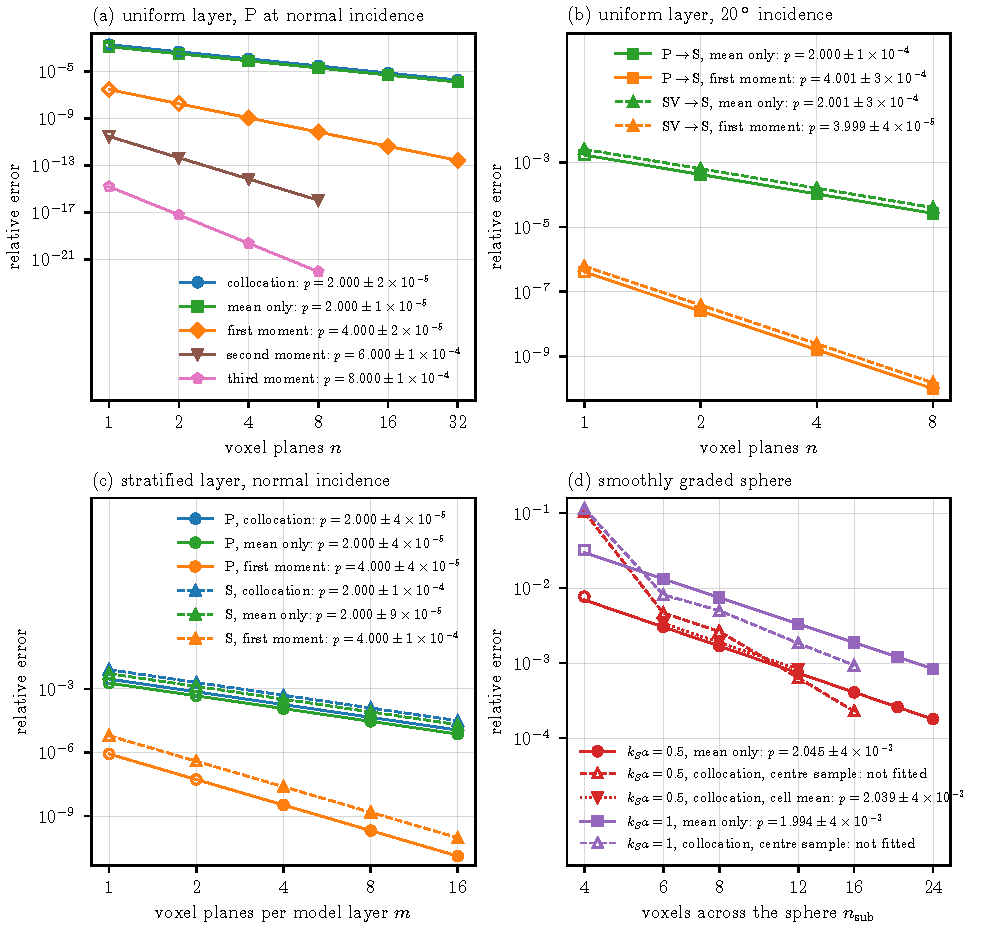
\includegraphics[width=\linewidth]{../figures/fig_convergence.pdf}
\caption{Convergence of every test, with least-squares regression lines. Each line fits
$\log e=c-p\log n$ to the filled points; open points are pre-asymptotic and are not fitted. The legend
gives the order $p$ and its standard error. The marker, and in colour the hue, marks the scheme, so
that the figure reads in grey scale: collocation (circles; \S\ref{sec:single}),
the mean-only voxel (squares) and the voxels carrying Legendre moments to degree $p=1$ (diamonds), $2$
(triangles) and $3$ (pentagons) (Eqs.~\eqref{eq:galerkin} and \eqref{eq:bloch}). (a)~The uniform layer, P reflection at normal
incidence ($D=2$\,m, $\omega=300$\,rad\,s$^{-1}$, the contrast of \S\ref{sec:convergence}), fitted from
$n=4$; the collocation line is dashed and lies on the mean-only line, from which its constant differs
only by the factor $3/2$ of Table~\ref{tab:ratio}; the second- and third-moment voxels, computed in 40-digit arithmetic, fitted from $n=2$. (b)~The uniform layer at $20^\circ$, fitted from
$n=2$: the S wave converted from incident P (solid) and reflected from incident SV (dashed).
(c)~The stratified layer of \S\ref{sec:hetero}, reflection at normal incidence for P (solid) and S
(dashed), against the number $m$ of voxel planes per model layer, fitted from $m=4$. (d)~The
smoothly graded sphere of \S\ref{sec:sphere} against its exact solution, for $n_{\mathrm{sub}}$ voxels
across: the mean-only voxel, fitted from $n_{\mathrm{sub}}=6$ (at $4$ a voxel is as wide as the
graded shell); the collocation voxel with the contrast sampled at the cell centre, joined by dashed
lines and not fitted, since its two $O(h^2)$ errors of opposite sign leave no single order to fit;
and, at $k_Sa=0.5$, the same collocation voxel with the cell mean of the contrast, dotted, which
recovers second order.}
\label{fig:convergence}
\par\smallskip{\footnotesize\textit{Alt text:} Four log--log panels of relative error against refinement,
each showing data points and fitted straight lines with the fitted order in the legend. (a) Uniform layer
at normal incidence, 1 to 32 voxel planes: the collocation and mean-only lines have order 2.000, the
first-moment line order 4.000, falling from about $3\times10^{-7}$ to $2\times10^{-13}$; the second-moment
line has order 6.000 and the third-moment line order 8.000, over 1 to 8 planes, reaching about $10^{-22}$. (b) Uniform layer at 20 degrees,
1 to 8 planes: P-to-S and SV-to-S lines, order 2.00 for the mean-only voxel and 4.00 for the
first-moment voxel. (c) Stratified layer, 1 to 16 planes per model layer: P and S reflection, order 2.000
for collocation and mean-only, 4.000 for first moment. (d) Smoothly graded sphere, 4 to 24 voxels across:
two straight falling lines of order 2 for the mean-only voxel, for $k_Sa=0.5$ and $1$, from about
$10^{-2}$ and $3\times10^{-2}$ at 4 voxels to $2\times10^{-4}$ and $8\times10^{-4}$ at 24; two
dashed collocation curves starting near $10^{-1}$ at 4 voxels, dropping steeply to 6 and then
falling faster than the mean-only lines, crossing below them by 16 voxels; and a dotted line of order
2 for the cell-mean collocation voxel, close to the mean-only line.\par}
\end{figure}

\paragraph{What each basis is for} A voxel holds two functions, and the results give each basis its
part. The basis of the wavefield sets how well the voxel carries the field across itself: in a uniform
medium the scheme converges at order $2p+2$ with the constant $c_p$ of Eq.~\eqref{eq:cp}, for P and S
waves and at normal and oblique incidence alike. The basis of the medium sets how well the voxel
\emph{is} the medium: with degree $r$ the order is capped at $2r+2$ (Eq.~\eqref{eq:graded}). Neither can
make up for the other, and the second-order term shows why. The field scattered once is a copy of the
medium's profile, so the wavefield basis must carry the profile as well as the wave, and the error of
that term is the relative projection error of the profile at the lower of the two degrees
(Eq.~\eqref{eq:defectlaw}). At the frequencies of interest the wave varies little across a cell and the
medium may vary much, so it is the medium, not the wavelength, that decides the degree and the size of
the cells. Two cases bracket the choice. Where the medium is piecewise constant on the cells, as in a
layered model with voxel faces on its interfaces, a constant is exact for the medium, the projection
error vanishes, and the degree of the field is spent entirely on the wave. Where the medium varies
smoothly within the cells, the two degrees should be equal: a higher degree for the contrast than for
the field is wasted, and a higher degree for the field improves only the Born term. That the two
degrees can be chosen independently is the practice of higher-order electromagnetic volume methods
\citep{Chobanyan2015}; what the present results add is the rule for choosing them, and the error each
choice leaves.

\paragraph{Where the error of a voxel scheme lives} The results separate the two approximations
a voxel scheme makes. The \emph{coupling} between voxels makes none: averaged over the source cell it
is the continuum's cell integral exactly, between planes by the form factor's zeros and within a
plane by the tiling identity, and the self term it omits is exactly the one the single site
carries. Every error therefore comes from the \emph{single site}: from the internal field it
assumes and, where the medium varies within the cell, from the medium it is given. Its $T$-matrix sums
the rescattering within the voxel exactly, but for the voxel as represented, and the split of the
second-order term in \S\ref{sec:hetero} measures the consequence: the error sits in the part whose two
scatterings lie in one cell, and the part between cells carries at most $0.2\%$ of it. For a uniform field that error is the midpoint rule's, known in closed form; for a linear
field it is the next term of the same expansion. The converse is the practical warning. A kernel that
is not the cell integral (the point Green's tensor, or a cell average that does not match the
single site's closure) leaves a local term that does not vanish as the voxels shrink
(\S\ref{sec:point}): the evanescent lattice orders carry a static contribution of fixed size per
voxel volume. A scheme built that way converges to the wrong limit, and refinement cannot reveal
it, because the error is scale-invariant.

\paragraph{What the single site is} The moment hierarchy of \S\ref{sec:single} turns the
uniform-field single site from a modelling choice into a derived object with a stated error. Its
static part is exact for a sphere, and for a cube it differs from the sphere's only by the cubic
split of Eq.~\eqref{eq:shearsplit}. Its dynamic part departs from exact scattering by a sphere only
through the real $(ka)^2$ term of Eq.~\eqref{eq:spheredynamic}; the radiation damping is exact.
That term and the collocation error of Eq.~\eqref{eq:errorR} have the same origin, the variation of
the field across the scatterer, and the same remedy, a richer internal field. In a lattice the
remedy is cheap: the field a voxel must represent is the smooth continuum field, not the field of an
isolated cube, with its concentrations at the edges and corners.

\paragraph{Relation to the coupled-dipole method} The same partition appears in the
coupled-dipole method as the choice of polarisability. The Clausius--Mossotti relation, the lattice
dispersion relation \citep{Draine1993}, the polarisability taken from the exact static solution
\citep{Rahmani2002} and the integrated Green tensor \citep{Chaumet2004} all adjust the single site
so that the lattice reproduces the continuum. For space-filling cubes the adjustment is neither
needed nor a free parameter: the tiling identity fixes the local field exactly, the self term of the
collocation closure is the one that makes it cancel, and what is left is a closed-form error rather
than an empirical one. That the method is a collocation of the volume integral equation was shown
for the electromagnetic case by \citet{Lakhtakia1992}; Eq.~\eqref{eq:collocation} is the same
statement for the elastic lattice with the self term evaluated over the finite cube, and it is what
makes the error a midpoint-rule error. The filtered coupled dipoles of \citet{Piller1998} and
\citet{Yurkin2010} band-limit the source to the grid; the source-cell average does the
complementary thing exactly, its form factor vanishing on the reciprocal lattice, and the spectral
construction of Eq.~\eqref{eq:bloch} is the periodic coupled-dipole method of \citet{Chaumet2003}
with the Galerkin double average in place of the point dipole. The second-order convergence
reported for the DDA by \citet{Yurkin2006} corresponds to the uniform-field voxel's, and the
opposite-signed constants of Eq.~\eqref{eq:errorR} explain why a polarisability correction can
improve one observable only at the expense of another, as the package's own form-factor corrections
do in reflection and transmission. Going beyond second order requires a richer internal field, which
is the point of higher-order bases for volume integral equations
\citep{Chobanyan2013,Georgakis2020}; the first-moment voxel is the
lowest such basis, and in its spectral form the Galerkin double average makes the lattice sum
converge without Ewald splitting.

\paragraph{The tension between the two error sources} The coupled-dipole method has two sources
of error, the single site and the coupling between sites, and each has been corrected on its own:
the polarisability by the Clausius--Mossotti relation, the lattice dispersion relation or the exact
static limit, and the coupling by integrating or filtering the Green tensor. The two are not
independent. The point kernel's evanescent orders carry a static local term whose size per voxel
volume does not shrink with the voxels (\S\ref{sec:point}), and the single site must cancel exactly
that term. A polarisability tuned for one kernel is therefore wrong for another: the lattice
dispersion relation corrects the point-dipole lattice, and changing the kernel to an integrated or
a filtered one changes the term it must cancel. Tuning either alone moves the error between the
two, and refinement cannot reveal a mismatch, because the surviving term is scale-invariant. For
space-filling cubes the tension is resolved rather than balanced: the cell-averaged kernel omits
exactly the self term that the closure carries (Eq.~\eqref{eq:collocation}), so the coupling error
vanishes identically and every remaining error is the single site's, the variation of the field
across the cell. That error has a second tension of its own. It is a midpoint-rule error whose
constants have opposite signs in reflection and transmission (Eq.~\eqref{eq:errorR}), so any
scalar adjustment of the single site that improves one worsens the other; the package's far-field
corrections reduce the reflection error by a factor $4.45$ and increase the transmission error by
$1.7$. No polarisability, however chosen, can remove it. What removes it is a richer internal
field: the first moment lowers the error by two orders in $kd$ in both observables at once.

\paragraph{The cost of fourth order} A first-moment voxel carries four times as many unknowns as
a uniform one (36 against 9 in three dimensions). The closed forms show what that buys. To reach an
error $\varepsilon$ in reflection, the uniform voxel needs $kd=\sqrt{8\varepsilon}$ and the
first-moment voxel $kd=(720\,\varepsilon)^{1/4}$; at $\varepsilon=10^{-6}$ that is $kd=2.8\times
10^{-3}$ against $0.16$, voxels $58$ times larger in each direction. In a three-dimensional model the
voxel count falls by $58^3\approx2\times10^5$ and the number of unknowns by about $5\times10^4$
(these are the Born-order constants; at the contrast studied the first-moment voxel's measured errors
lie within $5\%$ of them, while the uniform voxel's transmission constant grows with the contrast, so
the comparison is if anything conservative).
The stratified model of \S\ref{sec:hetero} measures it directly: $347$ planes of uniform-field voxels
against $8$ first-moment voxels for the same accuracy. Higher moments continue the trend in one
dimension: by Eq.~\eqref{eq:cp} the second-moment voxel reaches $\varepsilon=10^{-6}$ at $kd=0.68$ and
the third-moment voxel at $kd=1.5$, where a voxel is already a quarter of a wavelength. In three dimensions, with the Legendre products of total degree at most $p$, a voxel carries $10$
($p=2$) or $20$ ($p=3$) weights per state component, against $4$ for the first-moment voxel. The voxel
of degree $2$ converges at sixth order in the layer at oblique incidence (Table~\ref{tab:deg2}); that of
degree $3$ has not been built in three dimensions. The gain is largest precisely where it matters: when the model varies on scales that are coarse
compared with the accuracy the wavefield must have.

\paragraph{Limitations and outlook} The results concern laterally uniform media, a homogeneous layer
and a randomly stratified one, for which the discrete system is exactly a chain of planes; a laterally heterogeneous medium needs the
first-moment voxel in a full three-dimensional solver, where the gradient channels couple through
the evanescent lattice orders (\S\ref{sec:fourth}) and the tiling identity holds only to
$O(k_\parallel h)$. The smoothly graded sphere of \S\ref{sec:sphere} shows the mean-only
voxel converging at second order on a laterally heterogeneous body against an exact solution, and the
companion paper \citep{NestorGraded2026} shows the first-moment voxel converging at fourth order there.
A contrast that varies within a cell, which \S\ref{sec:hetero} shows is needed beyond second order in a
smoothly varying medium, has a further consequence in three dimensions: its linear part is odd about
the cell's centre, so it couples the single site's uniform-field and first-moment blocks, which parity
keeps apart for a homogeneous cube (\S\ref{sec:parity}). A graded voxel therefore needs at least the
first-moment block; that voxel is built, and tested on the graded sphere, in the companion paper. The numerical evidence is at moderate, physically typical contrasts (up to
$15\%$ in density and moduli) and at $k_Sh\le0.3$, the range in which the single-site $T$-matrix is
validated; the closed forms are first order in the contrast, and the departures from them at the
full contrast are of second order. What is established is the \emph{order} of convergence and its
leading constant, not the behaviour at strong contrast, where the single site's own closure may
limit the accuracy before the lattice coupling does. The single site's dynamic error is in closed
form for a sphere only; for a cube, for which no exact solution exists, it is known through the
layer (\S\S\ref{sec:convergence}--\ref{sec:fourth}). Two extensions follow directly. The first is
the three-dimensional solver itself. The second is a stratified \emph{background}, a layered
reference medium, as distinct from the stratified contrast of \S\ref{sec:hetero}. There the lattice coupling
then carries the reverberation of the layering, which is not translation invariant in depth, and
whether a tiling identity holds for it is the natural next question.

\section{Conclusions}\label{sec:summary}

A voxel of a volume-integral scheme must represent the medium within it and the wavefield within it.
This paper has determined what each basis must be and what error a given choice leaves, by an
experiment in which nothing else is approximated: a layer of cubes is the layer itself, so its exact
solution isolates the discretisation error.

With the wavefield expanded to Legendre degree $p$ and the contrast of the medium to degree $r$ in each
voxel, the scheme converges at order $\min(2p+2,2r+2)$. In a uniform layer the leading error is
$c_p(kd)^{2p+2}$ with the closed-form constant of Eq.~\eqref{eq:cp}, and a single plane of such voxels
reproduces the thin-layer series term by term through $O(D^{2p+2})$; the orders $2$, $4$ and $6$ of the
degrees $0$, $1$ and $2$ hold for P, SV and SH waves at normal and oblique incidence. The first-moment
voxel's leading error, $-(kd)^4/720$, does not depend on the direction of observation, whereas the
collocation scheme's is opposite in sign in reflection and transmission, so that no scalar correction of
the single site removes it. Where the medium varies within a cell, a contrast held constant caps every
voxel at second order, the coupling for a contrast of degree $r$ needs nothing beyond the same kernel
moments to degree $p+r$, and the error of the term of second order in the contrast is the relative
projection error of the medium at degree $\min(p,r)$, exactly in the long-wave limit. That error is the
single site's: its $T$-matrix sums the rescattering within a voxel exactly for the voxel as represented,
and the represented voxel is not the medium. The two bases must therefore be matched. Where the medium
is piecewise constant on the cells the projection error vanishes: the orders survive the interfaces of a
randomly stratified model, provided voxel boundaries coincide with them, and there the first-moment
voxel reaches an accuracy of $10^{-6}$ with one voxel per model layer, where the uniform-field voxel
needs about forty. A sphere whose contrast falls smoothly to zero at its surface converges at second
order against its exact solution, as the layer predicts, to $0.018\%$ at $k_Sa=0.5$ with twenty-four
voxels across; a sharp sphere's error is set by its staircase, which changes with the grid.

Three properties of the cube make the experiment exact. Because cubes tile the plane, the
source-cell-averaged coupling between voxels is the continuum's cell integral exactly, and at normal
incidence the lattice kernel is available in closed form with no lattice sum. The single site is derived
rather than assumed: the moments of the Green's tensor over the cube, taken as distributions, give a
closed hierarchy whose first-gradient truncation is the uniform-strain closure. That closure is exact
for a sphere in the static limit, it departs from exact scattering by a sphere only by a real $(ka)^2$
term, with the radiation damping exact, and for a cube it differs from the sphere only by a cubic
anisotropy of the shear response. And the collocation closure carries the same self term as the lattice
kernel, which cancels, so the discrete system is a collocation of the continuum equation, whose
second-order error is a midpoint-rule error of the internal field, known in closed form for every
discretisation. The results, and the evidence for each, are collected in Table~\ref{tab:evidence}.

\begin{table}[htbp]
\centering
\caption{The results of the paper, and the evidence for each.}\label{tab:evidence}
\begin{tabular}{@{}>{\raggedright\arraybackslash}p{0.52\linewidth}>{\raggedright\arraybackslash}p{0.40\linewidth}@{}}
\toprule
Result & Evidence \\
\midrule
Continuous layer, exact and to $O(D^k)$ & reference to $2.5\times10^{-8}$; series order $k$ \\
Thin-layer series, Eq.~\eqref{eq:thin} & each coefficient symbolically, to $D^4$ \\
Point-kernel local term survives $d\to0$ & $11\times$ the continuum term at $m=1$ \\
Averaged coupling between planes $=$ continuum$\times\sinc$ & $2.8\times10^{-16}$, 81 entries \\
Tiling identity, Eq.~\eqref{eq:tiling} & 21/21 components to $4\times10^{-9}$ \\
Exact kernel, Eq.~\eqref{eq:exactkernel} & replaces a $9.4\times10^{-4}$ static error \\
Moments as distributions, Eq.~\eqref{eq:peel} & sum rule \eqref{eq:sumrule} exact; $\mathsf M$, $\mathsf Q$ equal an independent archive, 81/81 \\
Channels \eqref{eq:A1g}--\eqref{eq:Eg} & a production code by another route, $2\times10^{-15}$ \\
Cube vs sphere, Eq.~\eqref{eq:shearsplit} & symbolic; and numerically at five $\nu$, $4\times10^{-16}$ \\
Ball closure $=$ exact Mie, static & $2\times10^{-10}$; cube's bulk and shear average $10^{-8}$ \\
Ball closure vs Mie, dynamic, Eq.~\eqref{eq:spheredynamic} & symbolic; numerical Mie $5\times10^{-4}$;
$(ka)^3$ terms exact \\
Self term cancels, Eq.~\eqref{eq:collocation} & $4\times10^{-16}$ \\
Package $T$ $=$ closure statically & $2\times10^{-5}$ at $k_Sh=0.01$ \\
Second-order convergence & order $2.000$, three frequencies \\
Closed-form error, Eq.~\eqref{eq:errorR} & $n=1$--$16$, to $10^{-4}$ of the error \\
First-moment voxel, Eq.~\eqref{eq:galerkin} & order $4.00$, three frequencies \\
First-moment voxel, oblique, Eq.~\eqref{eq:bloch} & order $4$, P and S, $20^\circ$ and $40^\circ$ \\
Incident SV and SH, all schemes & orders $2$ and $4$; constants with $k_S$ to $4\times10^{-4}$ \\
First-moment error $-(kd)^4/720$, Eq.~\eqref{eq:ratio} & $n=1$--$8$, to $10^{-4}$ of the error \\
Voxel of degree $p$: order $2p+2$ & $6.00$ ($p=2$, three frequencies), $8.00$ ($p=3$) \\
Constant $c_p$, Eq.~\eqref{eq:cp} & symbolic, $p=0$--$5$, twice; chain to $4\times10^{-7}$ \\
One plane of degree $p$ $=$ thin-layer series to $D^{2p+2}$ & exact series, $p=0$--$3$, two layers; $D^{3.00}$, $D^{5.00}$, $D^{7.00}$ \\
Independent implementation, any degree & within round-off; orders $4.02$, $6.02$ \\
Independent implementation of Eq.~\eqref{eq:bloch} & $1.1\times10^{-15}$, 40 cases: P, SV, SH, stratified \\
Random stratified layer, \S\ref{sec:hetero} & orders $2$ and $4$, P and S, normal and $20^\circ$ \\
Stratified reference against Kennett's recursion & $10^{-14}$ \\
Contrast varying within a cell, Eq.~\eqref{eq:graded} & $8$ cases, linear and smooth profiles; closed forms tested one by one to $2\times10^{-16}$ \\
Projection-error law, Eq.~\eqref{eq:defectlaw} & nine pairs $(p,r)$ to $1.3\%$; departure as $(kD)^2$; pairing symbolic, nine pairs \\
The error of $T_2$ is the single site's & same-cell part $0.998$ to $1.013$ of the law; between cells $\le0.002$ \\
Degree $2$ at oblique incidence, Table~\ref{tab:deg2} & order $6$, P, SV and SH, against Kennett's recursion \\
Smoothly graded sphere, \S\ref{sec:sphere} & exact solution by two routes, $2\times10^{-11}$; orders $2.04$ and $1.99$, $n_{\mathrm{sub}}=6$ to $24$ \\
\bottomrule
\end{tabular}
\end{table}

\paragraph{The error is known in advance} For every discretisation studied here the error is not
something to be discovered by refining until the answer stops changing. Its order and its leading
constant are known before anything is computed: $+(kd)^2/8$ in reflection and $-(kd)^2/24$ in
transmission for the collocation voxel (Eq.~\eqref{eq:errorR}), $(kd)^2/12$, $(kd)^4/720$ and
$(kd)^6/100800$ for the voxels of degree $0$, $1$ and $2$ (Eq.~\eqref{eq:cp}), and the order
$\min(2p+2,2r+2)$ where the medium varies within a cell (Eq.~\eqref{eq:graded}), with the size of the
error there given by the relative projection error of the medium (Eq.~\eqref{eq:defectlaw}), which is
computed from the model and the grid alone. That is worth more than
the order alone, for three reasons. First, the cell size and the degree of the voxel that a required
accuracy needs follow from the wavenumber and the medium, before the computation and without a
refinement study. Secondly, it turns a refinement study from a hope into a test. A scheme of this kind
can converge smoothly to the wrong limit (\S\ref{sec:point}), and smooth convergence alone cannot
reveal it; but the difference between two grids must have the known order and the known constant, and
a computation whose differences do not is in error from some cause other than the discretisation.
Thirdly, it shows where effort pays. The error is that of representing the field and the medium within
a cell, so raising the degree of the cell does what multiplying the cells cannot: in the stratified
model one first-moment voxel per layer reaches $10^{-6}$ where the uniform-field voxel needs about forty.
Whether the error of a body with three-dimensional structure can be known in advance in the same way is
the question taken up in the companion paper \citep{NestorGraded2026}.

\section*{Acknowledgments}
This work began thirty years ago in the author's doctoral research at the Research School of Earth
Sciences of the Australian National University, Canberra \citep{Nestor1996}.

\section*{Declaration of competing interest}
The author declares no known competing financial interests or personal relationships that could have
appeared to influence the work reported in this paper.

\section*{Declaration of generative AI and AI-assisted technologies in the manuscript preparation process}
During the preparation of this work, the author used Claude (Anthropic) in order to check the existing
Mathematica notebooks, Python and Fortran code, to build tests to ensure their correctness, and to
write the TikZ code of the diagrams. After using this tool, the author reviewed and edited the content
as needed and takes full responsibility for the content of the published article.

\section*{Data availability}
The Mathematica notebooks and Python scripts that derive and check every result, and the package they
test, are available at \url{https://github.com/tmnestor/MultipleScatteringCalculations}.

\bibliographystyle{elsarticle-num-names}
\bibliography{../references}

\end{document}
